%%!TEX encoding = UTF-8 Unicode

% Several lines in file have comments suggesting common packages for the
% typical thesis in informatics or electronics developed at UA
% uncomment/comment the lines as required for your work
% Before each optional line you will have a small comment

% According to UA rules, font size should range from 10 to 12pt.
\documentclass[11pt,a4paper,oneside,onecolumn]{memoir}

\listfiles
\fixpdflayout

\usepackage[utf8]{inputenc}

% Select Computer Modern Typewritter (For bold ttfamily in listings)
\usepackage{lmodern}
% OR... Bera Mono
%\usepackage[scaled]{beramono} % TTT Font
%\usepackage{anyfontsize} % As the name says...

\usepackage[T1]{fontenc}

% Enable for for Overleaf support
\usepackage{ifthen}
\def\useoverleaf{0}  % change to non-zero (for instance, 1) to enable it

\makeatletter
\newcommand{\makecoverfile}[0]{%
  \immediate\write18{latexmk -pdf cover.tex}%
}
\makeatother

% For PDF merging
\usepackage{pdfpages}

% Set DPI to 300
\pdfpxdimen=\dimexpr 1in/300\relax

% Allow the use of a larger number of packages
\usepackage{morewrites} 

% For English and Portuguese languages
% Portuguese will be the default.
% Uncomment \setlanguage below to change it
\usepackage[english,portuguese]{babel}

% Uncomment to use a custom date format
%\usepackage{datetime}
%\newdateformat{thesisdate}{\monthname[\THEMONTH] \THEYEAR} % Month Year

% Make pdf look better
\usepackage{microtype} 

% Uncomment to enable floats on facing pages
%\usepackage{dpfloat}

% Side by side figures
% Eg. Fig 1a, Fig 1b
\usepackage[hang,small,bf]{caption}
%\let\tion\undefined
%\let\subfloat\undefined
\usepackage{subcaption}

%\RequirePackage{textcase}

% Dropped Caps
%\usepackage{lettrine}

% Configure Hyperlink color
% As a matter or style, you may use this to enable/disable color boxes on links
%\usepackage[hidelinks,breaklinks=true,colorlinks=false,linkcolor=blue]{hyperref}
% Or use the default values provided by the hyperref package
\usepackage[hidelinks,breaklinks=true,colorlinks=false,linkcolor=blue]{hyperref}
% \usepackage{hyperref}

\usepackage{pgf-pie}

% Redefine section names according to your preference
%\def\sectionautorefname{Section}
%\def\chapterautorefname{Chapter}
%\def\figureautorefname{Figure}
%\def\listingautorefname{Listing}
%\def\tableautorefname{Table}

% Redefine code boxes
\ifthenelse{\equal{\useoverleaf}{0}}
{\usepackage[outputdir=build]{minted}}
{\usepackage{minted}}%

\addto\captionsportuguese{%
  \renewcommand\listingscaption{Código}
}
\fvset{fontsize=\footnotesize} % Make Code blocks smaller than text
\usepackage{csquotes}

% Add support for PDF Comments
\usepackage{comment}
\ifthenelse{\equal{\useoverleaf}{0}}
{\usepackage{pdfcomment}}{}
\usepackage{bookmark} % New Bookmarks

% For Multiple columns in Glossary
\usepackage{multicol}

% Add support for Math symbols
\usepackage{amsmath}
\usepackage{amssymb}

% Add support for graphics
\usepackage{graphicx}

% Add support for Colors
\usepackage{xcolor}

% Add support for the Euro symbol
\usepackage{eurosym}

% Add support for missingfigure and todo
\usepackage{todonotes}

% Setup bibliography with Biber using IEEE style for proper UTF-8 support
\usepackage[backend=biber, style=numeric, sorting=none, natbib=true, mincitenames=1, maxcitenames=2]{biblatex}
\bibliography{bib/references.bib}

% Define author-year citation command
\newcommand{\citeauthoryear}[1]{%
  \begingroup
  % \citeauthor{#1}, \citeyear{#1} \cite{#1}
  \citeauthor{#1} \cite{#1}
  \endgroup
}

% Use acronyms
\usepackage[printonlyused]{acronym} % For acronyms

% Indenting the first paragraph after section start
\usepackage{indentfirst}

% For fixing listoflistings with memoir
\usepackage{xparse}

% Uncomment the next lines to enable chart support through pgf and tikz
% This may require you to install further packages in your Tex system
%\usepackage[version=0.96]{pgf}
%\usepackage{tikz}

% UML support
%\usepackage{pgf-umlsd}

% Trees, Arrows, Mindmaps and other popular objects
%\usetikzlibrary{arrows,shadows,trees,shapes,decorations,automata,backgrounds,petri,mindmap} % for pgf-umlsd

% Package to master SI units
\usepackage[detect-weight=true, binary-units=true]{siunitx}
% For Electric Circuits
%\sisetup{load-configurations = binary}

% Set Voltage direction accordingly
% Option : oldvoltagedirection,nooldvoltagedirection,RPvoltages,EFvoltages
% More information at: https://mirrors.ibiblio.org/CTAN/graphics/pgf/contrib/circuitikz/doc/circuitikzmanual.pdf
% By default this template is using the Old Voltage Direction
%\usepackage[oldvoltagedirection,american,cuteinductors,smartlabels]{circuitikz}
%\usetikzlibrary{calc}
%\ctikzset{bipoles/thickness=1}
%\ctikzset{bipoles/length=0.8cm}
%\ctikzset{bipoles/diode/height=.375}
%\ctikzset{bipoles/diode/width=.3}
%\ctikzset{tripoles/thyristor/height=.8}
%\ctikzset{tripoles/thyristor/width=1}
%\ctikzset{bipoles/vsourceam/height/.initial=.7}
%\ctikzset{bipoles/vsourceam/width/.initial=.7}
%\tikzstyle{every node}=[font=\small]
%\tikzstyle{every path}=[line width=0.8pt,line cap=round,line join=round]

% For inline TT text (e.g. code snippets)
\usepackage{verbatim}

% Frames around figures and allow force placement
\usepackage{float}

% Configure Float style
%\floatstyle{boxed}
%\restylefloat{table}
%\restylefloat{figure}
%\restylefloat{lstlisting}

% For test purposes you may use the lipsum package to create dummy text
\usepackage{lipsum} % REMOVE

% Custom Packages
\usepackage{outlines}

%Keep floats inside section!
\usepackage[section]{placeins}
\let \oldsubsubsection \subsubsection
\renewcommand{\subsubsection}[2][]{
  \FloatBarrier
  \oldsubsubsection#1{#2}
}
\let \oldsubsection \subsection
\renewcommand{\subsection}[2][]{
  \FloatBarrier
  \oldsubsection#1{#2}
}
\let \oldsection \section
\renewcommand{\section}[2][]{
  \FloatBarrier
  \oldsection#1{#2}
}
\let \oldchapter \chapter
\renewcommand{\chapter}[2][]{
  \FloatBarrier
  \oldchapter#1{#2}
}



% Use the built-in division styling
\headstyles{memman}

% Include subsections in the TOC
\settocdepth{subsection}

% Numbering down to subsections as well
\setsecnumdepth{subsection}

% extra index for first lines
\makeindex[lines]

% Margins for University of Aveiro Thesis
\setlrmarginsandblock{3cm}{2.5cm}{*}
\setulmarginsandblock{3cm}{3cm}{*}
\checkandfixthelayout

% Or select your custom spacing to make any ajustment
%\addtolength{\parskip}{0.5\baselineskip}
\linespread{1.5}

\newcommand\mainmatterWithoutReset
{\edef\temppagenumber{\arabic{page}}%
  \mainmatter
  \setcounter{page}{\temppagenumber}%
}


%%%%%%%%%%%%%%%%%%%%%%%%%%%%%%%%%%%%%%%%%%%%%%%%%%
% Document begins here
%%%%%%%%%%%%%%%%%%%%%%%%%%%%%%%%%%%%%%%%%%%%%%%%%%

\begin{document}

% Fix the numbering scheme by having a ghost style for page numbering
\pagenumbering{Alph}

\ifthenelse{\equal{\useoverleaf}{0}}{}{\makecoverfile{}}%
\setcounter{page}{0}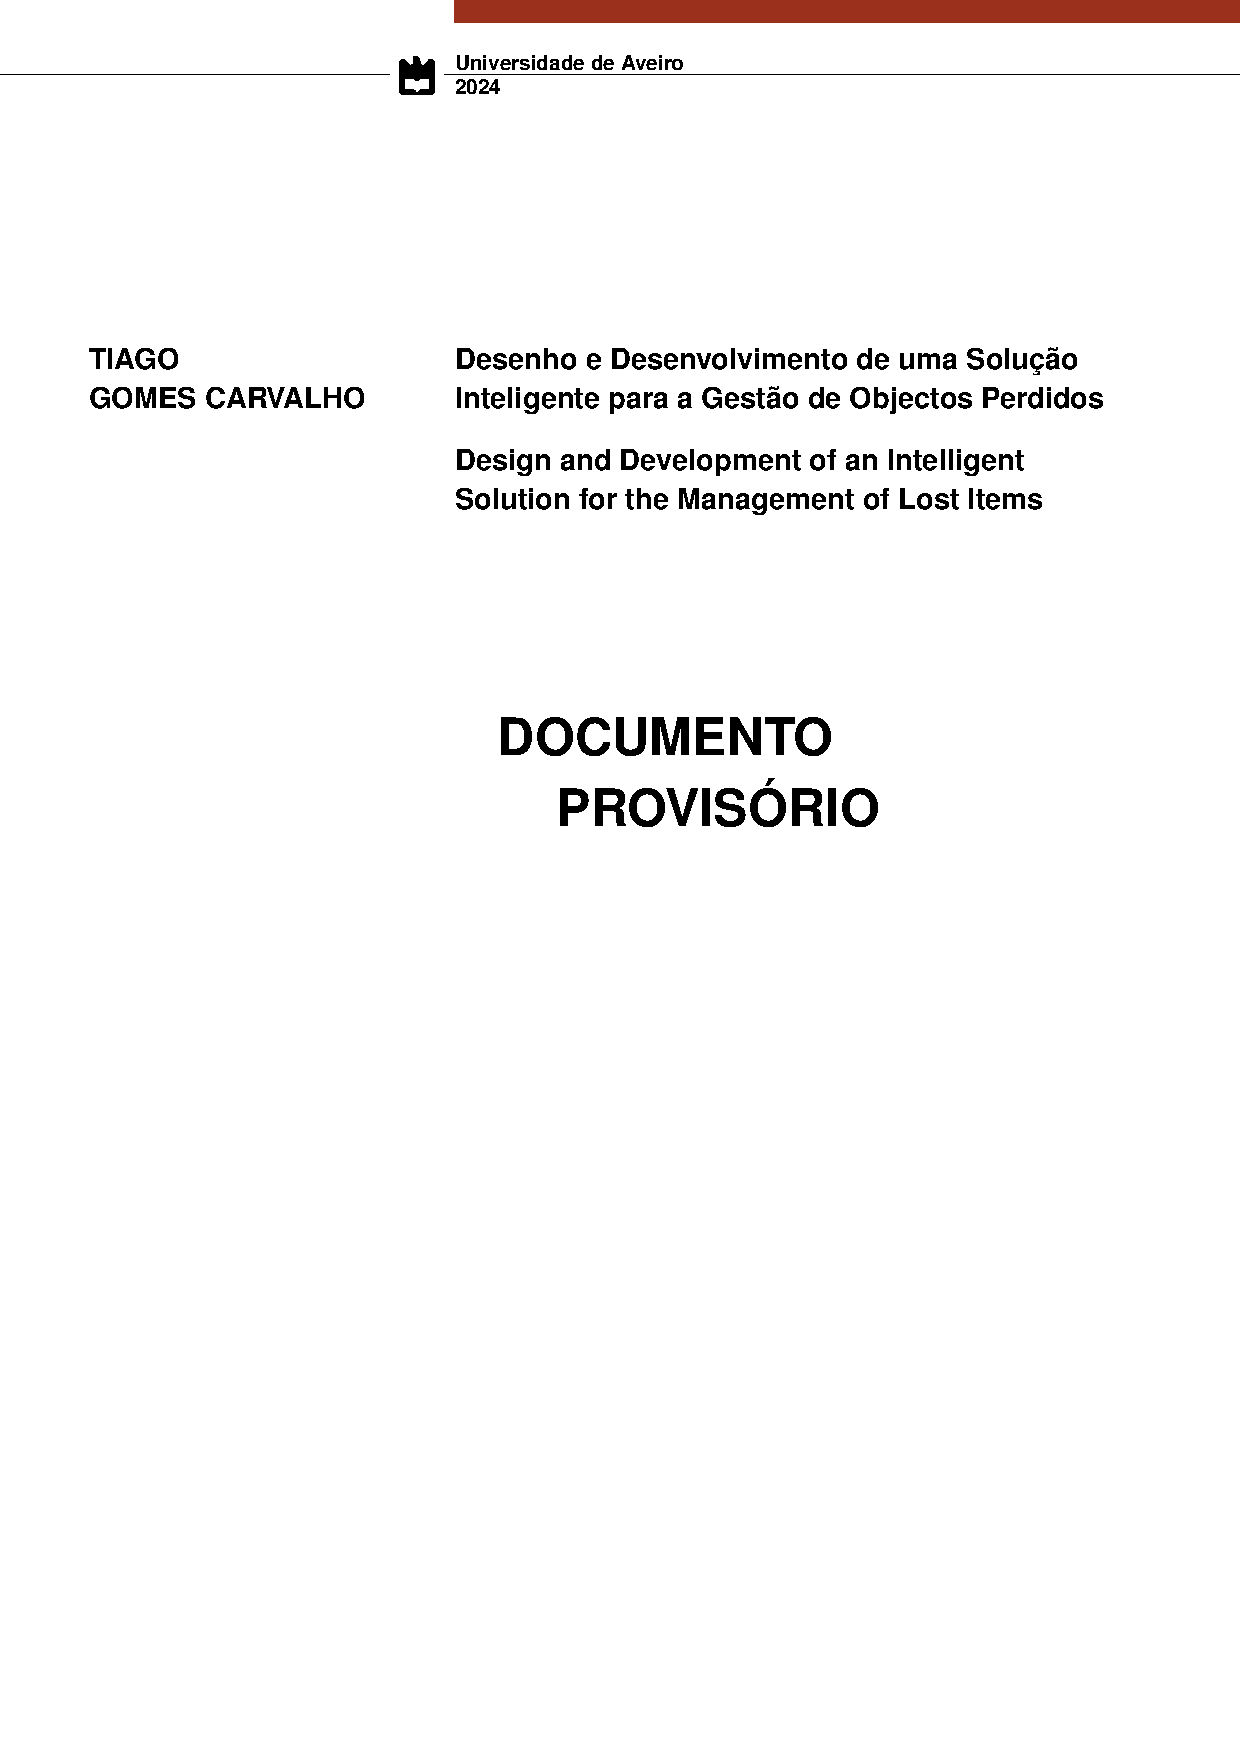
\includepdf[pages=-]{cover.pdf}

% Uncomment to enable English
\selectlanguage{english}


% Front matter

%Custom Chapter style named `thesis`
\makechapterstyle{thesis}{% Based on ell
  \chapterstyle{default}
  \renewcommand*{\chapnumfont}{\normalfont\sffamily}
  \renewcommand*{\chaptitlefont}{\normalfont\Huge\sffamily}
  \settowidth{\chapindent}{\chapnumfont 111}
  \renewcommand*{\chapterheadstart}{\begingroup
    \vspace*{\beforechapskip}%
    \begin{adjustwidth}{}{-\chapindent}%
    \hrulefill
    \smash{\rule{0.4pt}{15mm}}
    \end{adjustwidth}\endgroup}
  \renewcommand*{\printchaptername}{}
  \renewcommand*{\chapternamenum}{}
  \renewcommand*{\printchapternum}{%
    \begin{adjustwidth}{}{-\chapindent}
    \hfill
    \raisebox{10mm}[0pt][0pt]{\fontsize{30}{25}\selectfont\chapnumfont \thechapter}%
                              \hspace*{1em}
    \end{adjustwidth}\vspace*{-3.0\onelineskip}}
  \renewcommand*{\printchaptertitle}[1]{%
    \vskip\onelineskip
    \raggedleft {\chaptitlefont ##1}\par\nobreak\vskip 4\onelineskip}}


% Select chapter style from existing or select custom
%\chapterstyle{thesis} % Others: dowding, demo2, dash, chappell, brotherton, bianchi, ger, madsen, tatcher, veelo,indexes)
% thesis can also be used as defined previously
% Check the memoir documentation for the available themes
% Default is veelo
\chapterstyle{veelo}
\makeoddfoot{plain}{}{\thepage}{} % Added by André Zúquete to fix a page numbering issue on the veelo chapter style

% Select Page style
\pagestyle{plain}

% If you feel adventurous you can also define all aspects of your theme
% Use either this input or the chapterstyle before
% % Rules
\newcommand{\thinRule}{\rule{\textwidth}{0.25pt}}

% Customize heading appearances
% Define styles
\newcommand{\partSize}{\Huge}
\newcommand{\partStyle}{\lsstyle\scshape}
\newcommand{\chapterSize}{\Huge}
\newcommand{\chapterStyle}{\lsstyle\scshape}
\newcommand{\chapterAfter}{}
\newcommand{\sectionSize}{\Large}
\newcommand{\sectionStyle}{\scshape\MakeTextLowercase}
\newcommand{\subsectionSize}{\large}
\newcommand{\subsectionStyle}{\scshape\MakeTextLowercase}
\newcommand{\subsubsectionSize}{\large}
\newcommand{\subsubsectionStyle}{\scshape\MakeTextLowercase}
\newlength{\partNumSizePt}
\setlength{\partNumSizePt}{60pt}
\newlength{\chapterNumSizePt}
\setlength{\chapterNumSizePt}{60pt}
\newcommand{\partNumSize}{%
  \fontsize{\partNumSizePt}{1.2\partNumSizePt}\selectfont%
}
\newcommand{\partNumStyle}{\partChapterNumColor}
\newcommand{\chapterNumSize}{%
  \fontsize{\chapterNumSizePt}{1.2\chapterNumSizePt}\selectfont%
}
\newcommand{\chapterNumStyle}{\partChapterNumColor}

% Customize parts
\renewcommand{\partnamefont}{\partSize\partStyle}
\renewcommand{\partnumfont}{\partNumSize\partNumStyle}
\renewcommand{\printpartname}{}
\renewcommand{\printparttitle}[1]{%
  \normalfont\normalcolor\partnamefont #1
}

% Customize chapters
\makeatletter
\setlength{\beforechapskip}{30pt}
\renewcommand*{\chapterheadstart}{\vspace*{\beforechapskip}}
\setlength{\afterchapskip}{3ex}
\setlength{\midchapskip}{3ex}
\renewcommand*{\chapnamefont}{%
  \Large\flushright\chapterStyle\partChapterNumColor%
}
\renewcommand*{\chapnumfont}{\chapterNumSize\chapterNumStyle}
\renewcommand*{\chaptitlefont}{%
  \normalfont\flushleft\normalcolor\chapterSize\chapterStyle%
}
\renewcommand*{\printchaptername}{%
  \chapnamefont\MakeTextLowercase{\@chapapp}%
}
\renewcommand*{\chapternamenum}{\quad}
\renewcommand*{\printchapternum}{%
%  \chapnumfont\textls[-75]{\classicstylenums{\thechapter}}%
 \chapnumfont\textls[-75]{\thechapter}%

}
\renewcommand*{\printchaptertitle}[1]{%
  \chaptitlefont #1
  \chapterAfter
}
\makeatother
% Customize sections and subsections
\setsecnumformat{\csname my#1\endcsname\quad}
\setsecheadstyle{\sectionSize\sectionStyle}
\newcommand{\mysection}{{\thesection}}
\setlength{\beforesecskip}{3em}


\setsubsecheadstyle{\subsectionSize\subsectionStyle}
\newcommand{\mysubsection}{{\normalfont\subsectionSize\thesubsection}}
\setlength{\beforesubsecskip}{3em}

\setsubsubsecheadstyle{\subsubsectionSize\subsubsectionStyle}
\newcommand{\mysubsubsection}{{\normalfont\subsubsectionSize\thesubsubsection}}
\setlength{\beforesubsubsecskip}{2em}

% Customize "Table of ..." appearance
% Customize headings
\newcommand{\renewPrintXTitle}[1]{%
  \renewcommand{#1}[1]{%
    \printchaptertitle{##1}%
  }%
}
\renewPrintXTitle{\printtoctitle}
\renewPrintXTitle{\printlottitle}
\renewPrintXTitle{\printloftitle}

% Customize ToC headings
\renewcommand{\cftpartfont}{\partChapterNumColor\partStyle}
\renewcommand{\cftchapterfont}{\chapterStyle}
\renewcommand{\cftsectionfont}{}
\renewcommand{\cftsubsectionfont}{}
\renewcommand{\cftfigurefont}{}
\renewcommand{\cfttablefont}{}
\newcommand{\cftlstlistingfont}{}

% Increase number width
\newlength{\cftNumWidthIncrease}
\setlength{\cftNumWidthIncrease}{0.25em}
\addtolength{\cftpartnumwidth}{\cftNumWidthIncrease}
\addtolength{\cftchapternumwidth}{\cftNumWidthIncrease}
\addtolength{\cftsectionindent}{\cftNumWidthIncrease}
\addtolength{\cftsubsectionindent}{\cftNumWidthIncrease}
% No leader dots
%\renewcommand*{\cftpartdotsep}{\cftnodots}
%\renewcommand*{\cftchapterdotsep}{\cftnodots}
%\renewcommand*{\cftsectiondotsep}{\cftnodots}
%\renewcommand*{\cftsubsectiondotsep}{\cftnodots}
%\renewcommand*{\cftfiguredotsep}{\cftnodots}
%\renewcommand*{\cfttabledotsep}{\cftnodots}
%\newcommand*{\cftlstlistingdotsep}{\cftnodots}
% Set page numbers immediately after entry text
\newcommand{\tocEntryPageSep}{\hspace{1em}}
\renewcommand{\cftpartleader}{\cftdotfill{\cftdotsep}}
%\renewcommand{\cftpartafterpnum}{\cftparfillskip}
%\renewcommand{\cftchapterleader}{\tocEntryPageSep}
\renewcommand{\cftchapterleader}{\cftdotfill{\cftdotsep}}
%\renewcommand{\cftchapterafterpnum}{\cftparfillskip}
\renewcommand{\cftsectionleader}{\cftdotfill{\cftdotsep}}
%\renewcommand{\cftsectionafterpnum}{\cftparfillskip}
\renewcommand{\cftsubsectionleader}{\cftdotfill{\cftdotsep}}
%\renewcommand{\cftsubsectionafterpnum}{\cftparfillskip}
\renewcommand{\cftfigureleader}{\cftdotfill{\cftdotsep}}
%\renewcommand{\cftfigureafterpnum}{\cftparfillskip}
\renewcommand{\cfttableleader}{\cftdotfill{\cftdotsep}}
%\renewcommand{\cfttableafterpnum}{\cftparfillskip}
\newcommand{\cftlstlistingleader}{\cftdotfill{\cftdotsep}}
%\newcommand{\cftlstlistingafterpnum}{\cftparfillskip}
% Customize page numbers
\newcommand{\tocPageStyle}{\tocPageColor}
\renewcommand{\cftpartpagefont}{\tocPageStyle}
\renewcommand{\cftchapterpagefont}{\tocPageStyle}
\renewcommand{\cftsectionpagefont}{\tocPageStyle}
\renewcommand{\cftsubsectionpagefont}{\tocPageStyle}
\renewcommand{\cftfigurepagefont}{\tocPageStyle}
\renewcommand{\cfttablepagefont}{\tocPageStyle}
\newcommand{\cftlstlistingpagefont}{\tocPageStyle}

% Abstract
% Remove indents around abstract text
\setlength{\absleftindent}{0pt}
\setlength{\absrightindent}{0pt}
% Change font size to conform with the rest of the document text
\renewcommand{\abstracttextfont}{\normalsize}

% Customize headers and footers including page numbers
\newcommand{\hfTextSize}{\footnotesize}
\newcommand{\headTextStyle}{\lsstyle\scshape\MakeTextLowercase}
\nouppercaseheads
\makeevenhead{headings}%
             {\hfTextSize\thepage}%
             {}%
             {\hfTextSize\headTextStyle\leftmark}
\makeevenhead{plain}%
             {\hfTextSize\thepage}%
             {}%
             {\hfTextSize\headTextStyle\leftmark}
\makeoddhead{headings}%
            {\hfTextSize\headTextStyle\rightmark}%
            {}%
            {\hfTextSize\thepage}
\makeoddhead{plain}%
            {\hfTextSize\headTextStyle\rightmark}%
            {}%
            {\hfTextSize\thepage}


% Customize captions
\newcommand{\captionSize}{\small}
\newcommand{\captionStyle}{\scshape}
\newcommand{\captionWidthRatio}{0.9}

\captionnamefont{\captionSize\captionStyle}
\captiontitlefont{\captionSize}
\captiondelim{ -- }
\captiontitlefinal{}
\changecaptionwidth
%\captionwidth{\captionWidthRatio\textwidth}

% Define colors
%\newcommand{\titleColor}{\color[rgb]{0.616, 0.0627, 0.176}}
\newcommand{\titleColor}{\color[rgb]{0,0,0}}

\newcommand{\partChapterNumColor}{\titleColor}
\newcommand{\dropCapColor}{\titleColor}
%\newcommand{\tocPageColor}{\color[rgb]{0.0980, 0.329, 0.651}}

\newcommand{\tocPageColor}{\color[rgb]{0, 0,0}}
\definecolor{shade0}{rgb}{1.0 , 1.0 , 1.0 }
\definecolor{shade1}{rgb}{0.9 , 0.9 , 0.9 }
\definecolor{shade2}{rgb}{0.8 , 0.8 , 0.8 }
\definecolor{shade3}{rgb}{0.65, 0.65, 0.65}
\definecolor{shade4}{rgb}{0.45, 0.45, 0.45}
\definecolor{shade5}{rgb}{0.0 , 0.0 , 0.0 }



%Exclude sub figures from List of Figures
%\captionsetup[subfloat]{list=no}

% Texts
\newenvironment{introduction}
{%
  \begin{minipage}{\textwidth}%
   \itshape%
}
{%
  \end{minipage}%
  \par\addvspace{2\baselineskip plus 0.2\baselineskip minus 0.2\baselineskip}%
}

\frontmatter

\tightlists
\midsloppy
\raggedbottom

\setcounter{tocdepth}{2} %subsections are added to the TOC
\setcounter{secnumdepth}{4} %subsubsections are numbered

% Initial document tables start here: TOC, LOF, LOT, Glossary
% Table of contents with slightly smaller font
\cleardoublepage
{\small\tableofcontents}

% List of figures with slightly smaller font
\cleardoublepage
{\small\listoffigures}

% List of tables with slightly smaller font
\cleardoublepage
{\small\listoftables}

% List of code snippets

% Fix for Listings with memoir

\RenewDocumentCommand \chapter { s O{#3} m }{%
  \FloatBarrier
  \IfValueTF{#1}  % if optional star is seen
    {\oldchapter*{#2}}
    {\oldchapter#1{#2}}
}

%\renewcommand{\listingscaption}{Código}
%\renewcommand{\listoflistingscaption}{Lista de Excertos de Código}
%\clearpage
%{\small\listoflistings}
%\addcontentsline{toc}{chapter}{\listoflistingscaption}

% Reset Chapters
\renewcommand{\chapter}[2][]{
  \FloatBarrier
  \oldchapter#1{#2}
}

% Print Glossary
\cleardoublepage
{\small\chapter{Glossary}

\footnotesize
\DoubleSpacing

\begin{multicols}{2}
\begin{acronym}[]
	\acro{acdm}[ACDM]{Architecture-Centric Development Method}
	\acro{ai}[AI]{Artificial Intelligence}
	\acro{api}[API]{Application Programming Interface}
	\acro{cnn}[CNN]{Convolutional Neural Network}
	\acro{cors}[CORS]{Cross-Origin Resource Sharing}
	\acro{cpu}[CPU]{Central Processing Unit}
	\acro{crud}[CRUD]{Create, Read, Update, Delete}
	\acro{cv}[CV]{Computer Vision}
	\acro{dl}[DL]{Deep Learning}
	\acro{gdpr}[GDPR]{General Data Protection Regulation}
	\acro{http}[HTTP]{Hypertext Transfer Protocol}
	\acro{https}[HTTPS]{Hypertext Transfer Protocol Secure}
	\acro{ims}[IMS]{Inventory Management System}
	\acro{ip}[IP]{Internet Protocol}
	\acro{ir}[IR]{Information Retrieval}
	\acro{json}[JSON]{JavaScript Object Notation}
	\acro{jwt}[JWT]{JSON Web Token}
	\acro{llava}[LLaVA]{Large Language and Vision Assistant}
	\acro{lf}[LF]{Lost-and-Found}
	\acro{lfms}[LFMS]{Lost-And-Found Management System}
	\acro{llm}[LLM]{Large Language Model}
	\acro{ml}[ML]{Machine Learning}
	\acro{mq}[MQ]{Message Queue}
	\acro{mvp}[MVP]{Minimum Viable Product}
	\acro{nlg}[NLG]{Natural Language Generation}
	\acro{nlp}[NLP]{Natural Language Processing}
	\acro{nlu}[NLU]{Natural Language Understanding}
	\acro{pii}[PII]{Personally Identifiable Information}
	\acro{prisma}[PRISMA]{Preferred Reporting Items for Systematic Reviews and Meta-Analyses}
	\acro{rbac}[RBAC]{Role-Based Access Control}
	\acro{resnet}[ResNet]{Residual Neural Network}
	\acro{rest}[REST]{Representational State Transfer}
	\acro{rsr}[RSR]{Router-Service-Repository}
	\acro{html}[HTML]{HyperText Markup Language}
	\acro{slr}[SLR]{Systematic Literature Review}
	\acro{sop}[SOP]{Standard Operating Procedure}
	\acro{ssl}[SSL]{Secure Sockets Layer}
	\acro{ui}[UI]{User Interface}
	\acro{url}[URL]{Uniform Resource Locator}
	\acro{ux}[UX]{User Experience}
	\acro{xml}[XML]{eXtensible Markup Language}
	\acro{yolo}[YOLO]{You Only Look Once}
\end{acronym}
\end{multicols}

}

%%%%%%%%%%%%%%%%%%%%%%%%%%%%%%%%%%%%%%%%%%%%%%%%%%%%%%%
% Main document starts here
%%%%%%%%%%%%%%%%%%%%%%%%%%%%%%%%%%%%%%%%%%%%%%%%%%%%%%%

\mainmatter

% Line spacing: 1.5 pt 
\OnehalfSpacing

%%%%%%%%%%%%%%%%%%%%%%%%%%%%%%%%%%%%%%%%%%%%%%%%%%%%%%%
% Start of Thesis text 
%%%%%%%%%%%%%%%%%%%%%%%%%%%%%%%%%%%%%%%%%%%%%%%%%%%%%%%

% Uncomment to add further chapters
\chapter{Introduction}
\label{chapter:introduction}

\begin{introduction}
"We never discover the value of things till we have lost them"

- Dinah Maria Craik, A Life For A Life (1859)
\end{introduction}

\section{Context} \label{section:context}

The loss of personal items is a common situation that affects individuals in various contexts, from public spaces such as airports, universities and shopping centres \cites{Oke2017, Yao2019} to private institutions such as schools, companies and factories. On average, people misplace or completely lose up to nine items each week, with common culprits including mobile phones, keys, and sunglasses \cite{Prawira2024}. This distraction costs individuals from 15 to 50 minutes each day spent searching for these misplaced items \cites{Prawira2024, Knierim2012}. Over an average of 60 years of stated adult life, that implies approximately at least a total of 3680 hours (153,3 days) and 200 000 items misplaced or wholly lost \cite{Ahmad2015}. Adding to this issue, studies have revealed that the time spent searching for lost items can lead to financial losses that feel akin to literally throwing money away. The cumulative effect of these lost hours not only frustrates individuals but also impacts their financial well-being, a stark reminder of how daily distractions can drain both time and resources. These effects, when aggregated over long periods, also have alarming outcomes. The same studies also reveal a staggering annual waste of approximately \$177 billion dollars made by United State citizens \cite{Newswire2010} due to time spent searching for lost or misplaced items \cite{Ahmad2015}, which represents a figure that highlights a significant drain on productivity.

Traditionally, manually managing lost property has long been plagued by inefficiencies that disadvantage its corresponding stakeholders, i.e. the administrators and the individuals, both seeking to deliver and recover the lost belongings \cite{Sinha2024}. In most cases, the process relies heavily on manual efforts, requiring staff to record, store and track items using rudimentary tools such as paper records or basic spreadsheets. Others resort to simple and outdated \acp{ims} that are not designed to handle the complexities of lost property management \cite{Guinard2008}. This labour-intensive approach is time-consuming and prone to human error, leading to lost items, inaccurate records and miscommunication between departments or stakeholders \cite{Sinha2024, Guinard2008}. Additionally, most of the designated staff responsible for handling these tasks is rarely compensated or formally recognised for this additional responsibility. These employees are typically expected to manage lost items alongside their regular workload without extra pay, training, or resources \cite{Guinard2008}. They are tasked with organising found objects, responding to enquiries and ensuring that the rightful owners are identified, often with little or no support from automated or systematic processes, that divert attention from their core responsibilities and also foster frustration as they navigate an unsustainable workflow.

On the other hand, individuals searching for lost objects face many significant challenges. The lack of a standardised or intuitive system means they have to rely on guesswork or luck to recover their belongings. The stress is even more significant when they do not know where to start their search or if their lost object has already been found. It is the so-called "lost-and-found" effect, described by \citeauthoryear{Garling2023}, explaining the stressful mental process of over-valuing and prioritising the recovery of a missing item. The absence of transparent communication channels \cite{Guinard2008} or efficient recovery mechanisms further enhances this effect.

Complementing the ineffectiveness, the risks associated with poorly managed lost items are substantial. Without secure processes, lost objects are vulnerable to theft or unauthorised access \cite{Tan2023}. Identity theft and forgery become tangible threats when personal or sensitive belongings, such as identification documents or personal electronic devices, fall into the wrong hands \cite{Xue2022}. In addition, the public disclosure of personal information associated with lost property has become a concern that has not yet been the subject of a standardised solution \cite{Xue2022}. Furthermore, mismanagement can lead to legal complications, especially if disputes arise over lost objects that are improperly registered or not returned to the rightful owner. A prevalent issue with lost property platforms is the failure to establish a robust sense of trust among users \cite{Xue2022}. Specifically, there is often a lack of reliable assurance between the owner of the lost item and the finder. This vulnerability can lead to dishonest behaviour, including fraudulent claims or requests.

From an organisational point of view, even though some institutions provide designated \ac{lf} collection points \cite{Tan2023}, they also run the risk of damaging their reputation, potentially being held accountable and damaging relations with the communities they serve.

In a world where technology effortlessly simplifies our daily tasks, it is striking that we lack effective technological solutions for locating our physical belongings. This discrepancy highlights a critical gap in our everyday lives, underscoring the urgent need for innovative tools that can help us find our lost possessions efficiently.

\section{Motivation} \label{section:motivation}

Since managing lost objects still represents a common challenge, creating a more efficient system to solve this problem can ease the burden among users and the community. With more efficient \ac{lfms}, manual processes that are currently riddled with inefficiencies can be completely redesigned. Institutions can not only optimise recovery processes but also strengthen their commitment to user satisfaction, thus improving community relations and institutional reputation.

Emerging technologies such as \ac{ai}, \ac{nlp} and the increasing training and use of \acp{llm} offer unprecedented opportunities to address these challenges. \ac{ai} can facilitate the identification and categorisation of lost objects, while \ac{nlp} enables the use of users' interactions, such as searches and conversations, to extract relevant data \cite{Prawira2024}, which can then be used in the user's best interest. In recent years, the advent of \ac{dp} has revolutionised the performance of various visual tasks, leading to significant advancements in areas such as image classification \cite{Liu2022}. These improvements are not limited to mere accuracy; they encompass enhanced efficiency in processing large datasets, the ability to recognise intricate patterns, and the capability to generalise across diverse scenarios.

This dissertation is motivated by the potential of these technologies to innovate in an area that remains barely explored, aiming to transform the \ac{lf} management into an efficient, secure and user-friendly experience. The integration of these technologies can redefine the standards of lost objects' recovery and management, resolving inefficiencies and building trust among stakeholders. Beyond merely improving operational processes, a reimagined system for managing lost property must also emphasise community integration. By enabling direct communication between finders and owners, supported by platforms for community-based reporting, the solution can minimise reliance on intermediaries and streamline the recovery process. The community-oriented approach proposed by \citeauthoryear{Guinard2008} not only fosters trust among stakeholders but also encourages a culture of shared responsibility and collaboration, empowering users to take an active role in solving \ac{lf} challenges.

% A well-designed \ac{lfms} has the potential to extend its impact far beyond the immediate issue of misplaced belongings. By addressing the inefficiencies inherent in traditional processes and adopting a community-driven and technologically sophisticated approach, the proposed solution could serve as a model for innovation in related domains, offering a framework for reducing theft, enhancing data privacy, and fostering transparency, which can, in turn, bolster trust. Moreover, such a system represents a tangible demonstration of how intelligent technologies can address real-world problems, ultimately contributing to a more connected, efficient, and equitable society. In this way, solving the problem of lost property management not only resolves a long-standing challenge but also sets a precedent for the transformative power of technological solutions.

\section{Objectives} \label{section:objectives}

This research seeks to establish a straightforward framework for addressing the inefficiencies in the management of \ac{lf} property by defining specific and measurable objectives. A primary goal is to design and develop an intelligent \ac{ims} specialised for \ac{lf}, by exploring the application and capabilities of \ac{ai} and \ac{nlp} for automating the identification, categorisation, and recommendation of lost items, aiming to reduce manual workload and effectively complete the \ac{lf} cycle of items. Another objective is to prioritise usability by ensuring that the proposed solution accommodates individuals with varying levels of technological proficiency, which involves examining design strategies that promote accessibility and simplify interactions, fostering a more inclusive approach. The last objective is to include community-oriented features, which may encourage community engagement, emphasising on fostering direct communication between users. This engagement indicates that the level of user interactions will highly modify the user experience.

The research aims to employ iterative testing and validation in both controlled and real-world settings, including evaluating the system under diverse conditions. Consequentially, it implies the need to implement record-keeping and observability methods to generate actionable insights, enabling continuous improvement of the solution.

The proposed research can be conducted in four key stages, which align with a logical progression from understanding the problem to delivering a robust, focusing on different aspects of design and development.

\begin{enumerate}
    \item Study the State-of-the-Art: Review existing i) \acl{lfms}, ii) in-production solutions, iii) available and recommended technologies and iv) best practices and optimal approaches;
    \item Design the structure of the system by defining its architecture, features and workflows;
    \item Create the main system components, including all the planned features;
    \item Test the system in a real-world and controlled environment;
    \item Finalise and document the results for academic and practical use.
\end{enumerate}

\section{Dissertation Outline} \label{section:dissertation_outline}

This dissertation is structured into multiple chapters, each building upon the previous to provide a comprehensive understanding of the research and its outcomes. The document begins with this introductory chapter, Chapter  \ref{chapter:introduction}, that offers background information, including the core problem being addressed, the motivation for this research, and the objectives associated with the proposed solution.

Following this, Chapter \ref{chapter:state_of_art} examines the state of the art and explores topics such as traditional and modern \acp{lfms}; \ac{cv}, directly connected with the advances on \ac{ai}; \ac{nlp} and the use of \acp{llm} to perform \ac{nlu} tasks; and many others.

Chapter \ref{chapter:methodology} focuses on explaining the first design decisions for the platform, namely the architectural design that resulted in the notional architecture.

The following chapters are expected to cover the development of a proposed \ac{mvp}, the integration with the intelligent technologies, the results from the system's real-world testing, the system's quality assessment and the conclusions driven from this dissertation.

\chapter{State of Art}
\label{chapter:state_of_art}

\section{Manually Managing \acl{lf} Items} \label{sec:manually-managing-lf-items}

\subsection{Traditional Management Systems} \label{subsec:traditional-lf-systems}

Traditional \acp{lfms} typically relied on manual processes to log and manage items, sometimes papers or books and, in a few cases, spreadsheets \cite{Anas2023}. The fundamental components included physical logs, where details of found items - such as descriptions, location, and date of discovery - were recorded by staff or custodians.

Often, the responsibility of maintaining these records fell to a designated individual or department. Items were categorised and stored in a secure area, with the hope that owners would reclaim them. Matching found items to reported losses was a manual process, requiring significant time and effort \cite{Anas2023}. Descriptions provided by claimants were cross-referenced with recorded details to determine ownership. In some cases, rudimentary tagging systems were used to label items, aiding the identification process.

In environments like universities or corporate campuses, basic digital tools such as spreadsheets were usually introduced to track items. However, the overall workflow remained heavily dependent on manual oversight. Community bulletin boards, notices, or word-of-mouth were also standard methods to inform individuals about found items.

Despite their simplicity, these systems played a critical role in facilitating the return of lost belongings in the pre-digital era \cite{Mayura2024}. They fostered a sense of trust and collaboration within communities, relying on the goodwill and honesty of both finders and administrators. The traditional systems established the groundwork for modern approaches, providing valuable insights into the challenges and requirements of effective \ac{lf} management.

Despite the previously detailed inefficiencies of such systems, there are still those who would find these manual workflows to be more trustworthy. For some, the human element brings a level of accountability and understanding that automated systems cannot replicate. Manual processes allow for subjective judgment, which can be beneficial in complex scenarios where nuance is required. The tactile nature of handling paper documents or physical records fosters a sense of security and reliability. Moreover, people who have had negative experiences with technology might prefer traditional methods, viewing them as more stable and less prone to glitches or failures.


\subsection{Obstacles in Traditional Systems} \label{subsec:obstacles-traditional-systems}

While traditional \acp{lfms} have historically served their purpose in smaller or less demanding contexts, they face significant challenges when scaled to handle larger volumes of items or more complex environments \cite{Mayura2024}. The scalability of such systems is inherently constrained by their reliance on manual processes and both limited technological integration and automation.

A key obstacle is the dependency on human effort. As the number of items increases, so does the burden on staff, leading to delays, errors, and inefficiencies. In high-traffic environments, the sheer volume of items can quickly overwhelm even the most organised traditional systems. Without automation, processing and resolving claims becomes a time-intensive task, reducing the workflow's overall effectiveness. 

Another barrier to scaling is the lack of centralised data management. In traditional systems, records are often siloed, with each location or department maintaining its logs. Especially in larger organisations or distributed campuses, the absence of a unified database also impedes efficient reporting and analysis of trends, such as identifying frequent loss locations or categories of items.

Communication between stakeholders presents further challenges. Traditional systems often lack any mechanisms for notifying individuals about found items or updating claimants on the status of their reports, resulting in inefficiencies and frustrations, particularly in large-scale operations where the number of inquiries can be substantial.

Finally, the security of manual systems poses significant concerns. As the volume of items increases, the risk of theft, loss, or unauthorised access also rises. Inadequate labelling and verification processes can lead to disputes or errors in returning items to their rightful owners, further eroding trust in the system.

% These obstacles highlight traditional systems' limitations in adapting to the demands of modern \ac{lf} management. While effective in smaller, community-focused settings, their scalability issues underscore the need for innovative solutions that leverage technology to enhance efficiency, security, and user satisfaction.


\section{Inventory Management Systems} \label{sec:ims}

\acp{ims} are tools designed to manage and track inventory levels across various domains. These systems enable organisations to streamline their operations, reduce costs, and enhance customer satisfaction by ensuring the availability of necessary items at the right time and place \cite{Pauliina2024}. An \ac{ims} employs methodologies to identify and classify inventory items based deatails like quantity, volume, value or variability, optimising inventory performance through targeted strategies \cite{Pauliina2024}.

Fundamentally, an \ac{ims} aims to address some challenges, such as maintaining inventory levels, reducing holding costs, mitigating risks and many others associated with collections and stocks. Techniques like safety stock determination and lot-sizing methods have been widely adopted \cite{Prabakaran2023}. Such systems have historically evolved to incorporate some technological advancements, obtaining the capability to predict, plan, and execute inventory operations Automatically and effectively \cite{Chebet2019}.

While conventional \acp{ims} primarily focus on physical products, their underlying principles can be effectively applied to tracking and managing \ac{lf} items. This intersection becomes particularly relevant in environments where the inventory (in this case, lost items) exhibits variability in value, volume, and retrieval demand. Inventory management principles, such as classification and optimisation, can be applied to \acp{lfms} to streamline processes and enhance user experiences. For instance, using the classification method mentioned before, in a \ac{lfms}, items could be categorised using an adapted ABC-XYZ\footnote{Suryaputri Z. and Gabriel, D.S. and Nurcahyo R., Integration of ABC-XYZ Analysis in Inventory Management Optimization: A Case Study in the Health Industry, Proceedings of the International Conference on Industrial Engineering and Operations Management, 2020, \url{https://ieomsociety.org/proceedings/2022nigeria/70.pdf}}framework that enables prioritisation of storage, retrieval, and notification efforts \cite{Khobragade2018}. The Table \ref{tab:abc_xyz} illustrates a potential result of that association:

\begin{table}[H]
\centering
\caption{Classification of \ac{lf} items using the ABC-XYZ framework}
\begin{tabular}{|c|c|c|c|c|}
\hline
\textbf{Class} & \textbf{Value} & \textbf{Volume} & \textbf{Retrieval Demand} & \textbf{Examples} \\ 
\hline
A-X & High & Low & Consistent & Electronic devices, jewellery \\ 
\hline
B-Y & Moderate & Moderate & Fluctuating & Wallets, bags, clothing \\ 
\hline
C-Z & Low & High & Irregular & Umbrellas, stationery \\ 
\hline
\end{tabular}
\label{tab:abc_xyz}
\end{table}

The insights from \citeauthoryear{Plinere2016} further support the integration of these methodologies into \acp{lfms}. Their case study emphasises the significance of structured inventory management practices for improving operational efficiency. For instance, high-priority items, such as class A-X items, can benefit from focused attention and expedited claim processes, ensuring user satisfaction while reducing storage costs. Furthermore, their findings highlight the value of predictive analytics in addressing slow-moving or stagnant inventory, matching to unclaimed items \cite{Plinere2016}. Technological integration, as illustrated in the case study, offers another avenue for improvement. The use of \ac{rfid} and \ac{qr} codes in conventional inventory systems ensures accurate tracking and categorisation of items \cite{Plinere2016, Sohail2018}. Moreover, the adoption of resource planning principles, such as imposing a centralised warehouse, would improve transparency and decision-making, possibly enabling a seamless synchronisation of data across departments. Lastly, the \citeauthoryear{Plinere2016} study underlines the importance of standardisation in inventory management policies, e.g., uniform intake procedures, categorisation standards, and clear guidelines for item disposition.

Adapting \acp{ims} for \ac{lf} management would definitely address some unique challenges \cite{Pauliina2024}. Unlike traditional inventory, lost items often have sentimental value or urgent retrieval needs, requiring the system to incorporate real-time tracking and user-friendly interfaces. Moreover, integrating predictive analytics, commonly used in \acp{ims} for forecasting demand, would be leveraged to anticipate peak periods of item loss or retrieval, e.g., events or seasons that may influence the volume and types of items lost, allowing proactive resource allocation \cite{Prabakaran2023}.

Building on these foundational principles, open-source \acp{ims} have evolved to address specific needs, blending traditional methodologies with modern technologies to enhance their adaptability and utility across domains. Odoo Inventory\footnote{\url{https://www.odoo.com/app/inventory}}, for instance, exemplifies this progression by integrating inventory management with enterprise-level tools like sales and customer relationship management. Its multi-warehouse support and barcode scanning capabilities make it a robust solution for medium to large enterprises. In contrast, Snipe-IT\footnote{\url{https://snipeitapp.com/demo}} focuses on a narrower domain (asset tracking), offering a well-designed interface for managing fixed assets, albeit without features like demand forecasting or multi-warehouse management. Moving further into specialised territories, InvenTree\footnote{\url{https://inventree.org/}} demonstrates how inventory systems can cater to engineering and manufacturing by providing tools for managing parts and components through hierarchical structures and batch tracking. However, it lacks the scalability offered by integration with other systems. Meanwhile, SkuNexus\footnote{\url{https://skunexus.com}} exemplifies the pivot toward e-commerce needs, combining advanced reporting, omnichannel order fulfilment, and process automation for complex operations, though its configurability demands significant effort during implementation. For small-scale, niche applications, PartKeepr\footnote{\url{https://partkeepr.org/}} offers essential inventory management tools, such as batch tracking and stock alerts, tailored to managing electronic components but without the scalability or advanced features needed for more extensive operations.

The following Table \ref{tab:ims_comparison} summarises the key features of these systems, highlighting their areas of strength and limitations:

\begin{table}[!htb]
\centering
\caption{Summarised comparison of open source \acl{ims} by features}
\begin{tabular}{lllllll}
\hline
\textbf{\ac{ims}} & \textbf{MWS} & \textbf{BI} & \textbf{DF} & \textbf{BT} & \textbf{ERPI} & \textbf{UFI} \\
\hline
Odoo & Yes & Yes & Yes & Yes & Yes & Yes \\
\hline
Snipe-IT & No & No & No & No & No & Yes \\
\hline
InvenTree & No & Yes & No & Yes & No & Yes \\
\hline
SkuNexus & Yes & Yes & Yes & Yes & Yes & No \\
\hline
PartKeepr & No & Yes & No & Yes & No & No \\
\hline
\end{tabular}
\caption*{\\MWS - Multi-Warehouse Support, BI - Barcode Integration, DF - Demand Forecasting, BT - Batch Tracking, ERPI - ERP Integration, UFI - User-Friendly Interface.}
\label{tab:ims_comparison}
\end{table}


\section{\acl{slr}} \label{sec:literature-review}

\subsection{Research Question and Methods} \label{subsec:slr}

\ac{lf} management has historically presented numerous challenges across both public and private sectors, as highlighted in a wealth of academic articles and studies \cite{Prawira2024}. To address previously mentioned persistent issues and uncover effective solutions, a rigorous \ac{slr} was undertaken, focusing specifically on innovations, challenges, and best practices in the realm of intelligent lost property management. The review was designed with a methodological rigour that adheres to the PRISMA 2020 guidelines \cite{Page2021}, ensuring that every aspect of the research was conducted with the highest standards of integrity and transparency. By synthesising the latest uncovered findings, the \ac{slr} offers not only a comprehensive understanding of the current landscape but also valiable insights that can inform the design of a \ac{lfms} system. The \ac{slr} later resulted in the production of a document directly aligned with this dissertation's scope, named \textit{"Designing an Intelligent Solution for Lost Property Management: A Systematic Review"}.

The review sought to answer the central research question \textit{"How can intelligent technologies enhance the efficiency and user experience of lost property management systems?"}, which refers to how technologies such as \ac{ai}, \ac{nlp}, \ac{cv} and many others can provide solutions to the inefficiencies in \ac{lf} management. The \ac{slr} analysed numerous articles and integrated 18 high-quality studies that demonstrated the capacity to provide new insights into the investigation area. The mentioned research question was then separated into the following three major objectives:

\begin{itemize}
\item Evaluating the applicability of the selected technologies;
\item Examining existing challenges in implementing these technologies;
\item Identifying best practices to inform the design and development of a proposed system.
\end{itemize}

The \ac{slr} employed a comprehensive four-phase approach, associated with the selected PRISMA framework. During the identification phase, academic databases such as Scopus and Web of Science were queried using targeted keywords like \ac{lf} Management, \ac{ims}, \ac{ai}, \ac{nlp}, and \ac{llm}, resulting in an initial yield of 476 studies. These were screened for relevance through the removal of duplicates and an abstract examination. In the eligibility phase, full-text articles were meticulously assessed against predefined inclusion criteria, which focused exclusively on studies published between 2020 and 2024 that addressed ac{ai}-based solutions. Non-peer-reviewed works and studies lacking empirical validation were excluded. Additionally, to ensure the robustness of the \ac{slr}, a quality assessment framework evaluated the methodological rigour and relevance of each study. Each study was rated on its technological contributions and practical applicability. Only those scoring consistently high across all criteria were included. Ultimately, in the inclusion phase, 18 studies were selected and categorised based on the technologies employed. Figure \ref{fig:prisma} illustrates the PRISMA flowchart, summarising the selection process. A thematic analysis was conducted, extracting valuable results into the contributions of each technological domain.

\begin{figure}[!htb]
    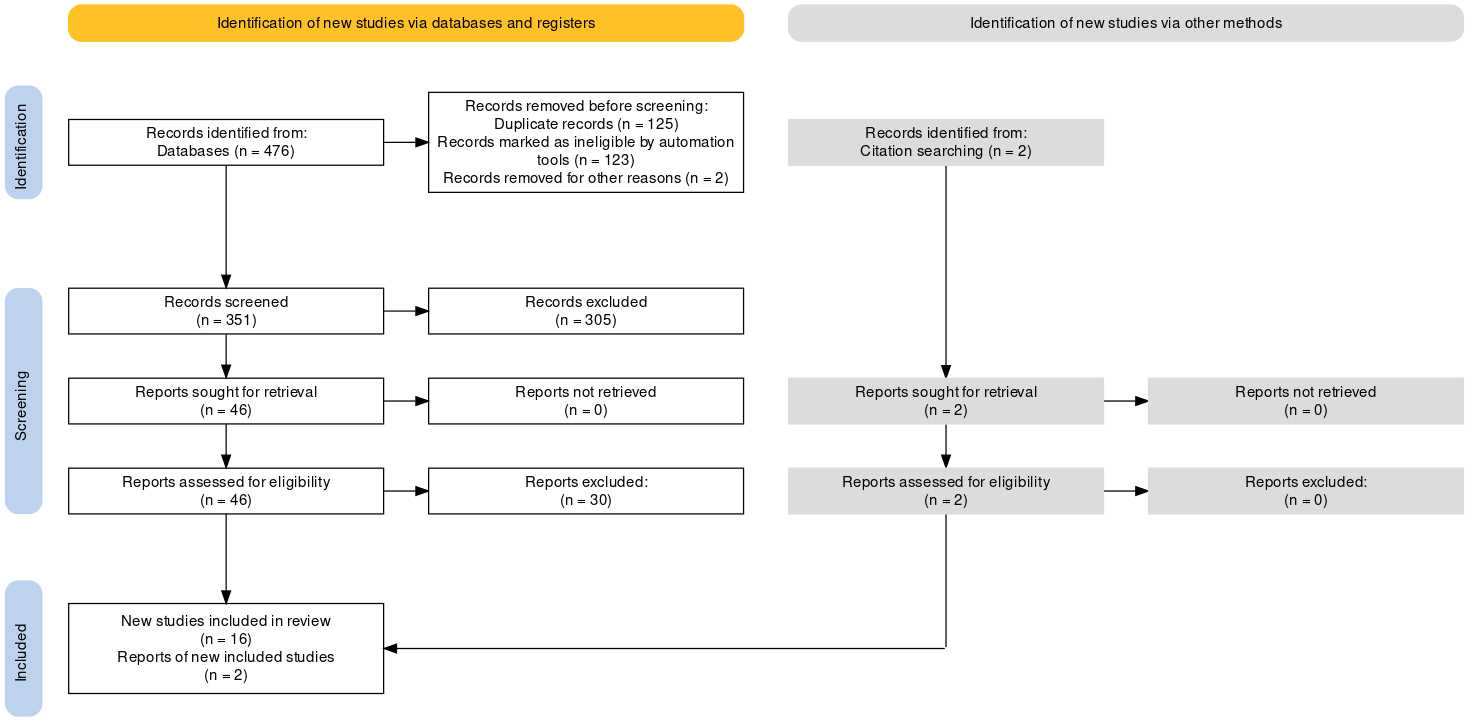
\includegraphics[width=0.95\textwidth]{figs/chapter2/prisma.png}
    \centering
    \caption[PRISMA flow diagram with a described quantity of research in each step.]{PRISMA flow diagram with a described quantity of research in each step.}
    \label{fig:prisma}
\end{figure}

\subsection{Object Recognition and Categorisation} \label{subsec:object-recognition}

Object recognition and categorisation are pivotal processes in the domain of \ac{ai} and \ac{cv}. Object recognition involves identifying objects within an image or video and distinguishing them based on predefined features. Categorisation goes a step further by grouping identified objects into classes and/or groups of classes based on shared attributes or relationships \cite{Liu2021}. These tasks are foundational to numerous applications, including autonomous vehicles, facial recognition, surveillance systems, and many others.

The origins of object recognition can be traced back to the early experiments in pattern recognition during the 1950s and 1960s. Early approaches relied heavily on rule-based systems, where objects were identified using manually defined features such as edges, corners, or textures. \citeauthoryear{Marr1982}'s seminal work on computational vision in the 1980s introduced the concept of multi-level processing, exposing the importance of integrating both low-level (e.g., edge detection) and high-level (e.g., semantic) features. The field evolved significantly in the 1990s with the advent of statistical methods and \ac{ml}. Techniques like support vector machines and decision trees provided more robust frameworks for categorisation \cite{Bishop2006}. Concurrently, datasets such as MNIST\footnote{\url{https://yann.lecun.com/exdb/mnist/}} and ImageNet\footnote{\url{https://www.image-net.org/}} emerged, enabling standardised benchmarking and driving advancements in recognition accuracy.

The evolution of object recognition and categorisation has been marked by the rise of \ac{dl} in the 2010s. \acp{cnn}, such as AlexNet\footnote{\ac{cnn} architecture, designed by Alex Krizhevsky in collaboration with Ilya Sutskever and Geoffrey Hinton at the University of Toronto in 2012} and \ac{resnet}, models capable of leveraging feature extraction, revolutionised this field by achieving human-like performance on challenging tasks. These models finally enabled the recognition of complex patterns and relationships in data \cites{He2015, Krizhevsky2017}. More recently, transformer-based architectures, exemplified by vision transformers, have further enhanced the capabilities of recognition systems. These models utilise attention mechanisms to capture long-range dependencies and contextual information, surpassing the limitations of traditional \acp{cnn} \cite{Dosovitskiy2020}.

\acp{cnn}, particularly \ac{resnet}-50, are widely utilised due to their capability to extract robust visual features. Studies have shown that ResNet-50 achieves high accuracy in identifying objects with varying attributes and appearances, a critical aspect for handling the heterogeneity of \ac{lf} items such as electronics, accessories, or apparel \cites{Prawira2024, Ghazal2016, Liu2022}. Similarly, \ac{yolo} models, including \ac{yolo}v7, are renowned for their real-time detection capabilities, ensuring low-latency processing and high precision even in challenging environments such as low light or cluttered backgrounds \cites{Sharma2024, Vedanth2024}.

\ac{resnet}-50, short for \acl{resnet} with 50 layers, has a \ac{dl} architecture designed to address the vanishing gradient problem in very deep neural networks. It introduces shortcut connections, or residual blocks, that allow gradients to flow more effectively during backpropagation, ensuring better convergence during training. \ac{resnet}-50 has become a standard in computer vision tasks due to its balance of depth and computational efficiency, making it suitable for extracting intricate visual features from diverse datasets \cite{He2015}. Its ability to generalise across object categories makes it a reliable choice for \ac{lf} management applications. \ac{yolo} is an object detection algorithm known for its speed and accuracy. Unlike traditional methods that scan an image region by region, \ac{yolo} processes the entire image in a single pass, predicting bounding boxes and class probabilities simultaneously, which significantly reduces computation time while maintaining high detection precision. \ac{yolo}v7, a more recent iteration, builds on these strengths by introducing architectural improvements for better performance in real-time scenarios, including high-density environments like traffic monitoring \cites{Redmon2015, Wang2022}.

Object recognition models can struggle with computational intensity, requiring significant resources for training and deployment \cites{Lubna2021, Mezhenin2021}. Lightweight versions of models are being developed to mitigate these issues, particularly for mobile applications, which are essential for systems designed to be universally accessible. Mobile-compatible frameworks, using optimised \ac{cnn}, provide the added advantage of enabling real-time item reporting and retrieval through user-friendly interfaces, expanding the reach of such systems \cites{Stout2024, Ghazal2016}.

Furthermore, these systems still need to contend with the diverse characteristics of objects. Items with subtle features or ambiguous shapes often pose difficulties for detection algorithms. Addressing this requires extensive and diverse datasets for training and validating in order to ensure that models can generalise effectively without overfitting to specific item categories \cites{Prawira2024, Liu2022, Sharma2024}. Hybrid approaches that integrate multiple algorithms or modalities are emerging as strategies to overcome these limitations. For instance, combining cloud-based data synchronisation with multimodal recognition has improved retrieval rates by facilitating large-scale processing and analysis \cite{Liu2024, Vedanth2024}.

\subsection{\acl{nlp}} \label{subsec:nlp}

\ac{nlp} is a multidisciplinary field at the intersection of linguistics, computer science, and artificial intelligence, enabling machines to process, understand, and generate human language. \ac{nlp} encompasses two core subfields: \ac{nlu} and \ac{nlg} \cite{Khurana2023}. \ac{nlu} focuses on interpreting and extracting meaning from textual or spoken language, including tasks such as sentiment analysis, intent recognition, and entity extraction, allowing systems to comprehend user input and respond accordingly \cite{Khurana2023}. In contrast, \ac{nlg} involves creating coherent and contextually appropriate textual or spoken output from structured data, such as generating summaries, reports, or conversational responses \cite{Dong2021}.

The origins of \ac{nlp} date back to the 1950s, when \citeauthoryear{Turing1950} proposed the concept of machine intelligence in his seminal work "Computing Machinery and Intelligence". One of the early milestones was the development of the Georgetown-IBM experiment in 1954, which demonstrated automatic translation between Russian and English, albeit limited to a small vocabulary and specific grammatical constructs. This marked the beginning of using computers to process and understand human language \cite{Hutchins2004}. About 50 years later, in the 1990s and early 2000s, \ac{ml} algorithms, mainly supervised learning, began to dominate \ac{nlp}, enhancing part-of-speech tagging, named entity recognition, and sentiment analysis. This era also witnessed the rise of the first large-scale resources for \ac{nlp}, including the Penn Treebank\footnote{https://catalog.ldc.upenn.edu/docs/LDC95T7/cl93.html} and WordNet\footnote{https://wordnet.princeton.edu/}, which provided valuable training data and lexical knowledge \cite{Marcus1993, Fellbaum1998}.

More recently, the new era has been characterised by a revolution in \ac{nlp} fueled by \ac{dl}. Neural network architectures, particularly recurrent neural networks and their derivatives, long short-term memory networks, demonstrated remarkable capabilities in sequence-to-sequence tasks such as translation and text summarisation \cite{Bahdanau2015}. Furthermore, the introduction of attention mechanisms and transformer-based models, such as \ac{bert} and \ac{gpt}, has drastically improved the state of the art, enabling unprecedented performance across a wide range of \ac{nlp} tasks \cite{Vaswani2017, Devlin2019}. Today, \ac{nlp} continues to evolve, integrating cutting-edge advancements in \ac{ai}, including transfer learning and pre-trained language models, to achieve higher accuracy and efficiency in a variety of complex tasks, namely sentiment analysis, machine translation, and conversational agents \cite{Howard2018}.

The systematic review highlights the growing role of \ac{nlp} in intelligent systems, particularly in enhancing human-computer interaction and automating complex processes. For instance, \ac{nlu} is central to enabling systems to interpret user input, extracting key entities, sentiments, and intents. \citeauthoryear{Prawira2024} and \citeauthoryear{Ghazal2016}, have already adopted these capabilities in their \ac{lfms} to streamline the reporting and retrieval of lost items. By leveraging \ac{nlu} models, their systems can process user descriptions into structured data that, once properly stored and indexed, can later be matched against found items.

Despite these advancements, several challenges remain. Scalability and computational efficiency are ongoing concerns, particularly when deploying \ac{nlp} models in real-time applications. Additionally, ethical considerations, including bias in language models and data privacy, require attention to ensure the responsible use of \ac{nlp} technologies \cite{Prawira2024}.


\subsection{Multimodal Matching} \label{subsec:multimodal-matching}

Embeddings play a pivotal role in modern artificial intelligence, particularly for applications requiring the integration of multimodal data such as images and text. These embeddings transform high-dimensional data into a lower-dimensional vector space while preserving semantic relationships. For example, image embeddings are often generated using \ac{cnn}, whereas text embeddings leverage transformer-based models \cite{He2015, Devlin2019}. This dimensionality reduction enables efficient and meaningful comparisons across large datasets.

Similarity search is a cornerstone technique in embedding-based systems. \citeauthoryear{Prawira2024} and \citeauthoryear{Ghazal2016} have experimented with metrics such as cosine similarity and Euclidean distance in order to quantify the proximity between embeddings, offering probabilistic measures of match likelihood between simulated \ac{lf} items. A high cosine similarity score, for instance, suggests strong alignment between query and database entries. Probabilistic models can further refine these measures, incorporating confidence intervals that guide the decision-making \cite{Dosovitskiy2020}.

Considering the domain of \ac{lf} management, embeddings would facilitate the matching of user-provided data to stored items or records. Visual embeddings derived from processed uploaded images would be compared against a database of known items. Similarly, textual embeddings generated from user descriptions and interactions could be matched to metadata or textual entries in the database. When combined, these approaches improve the accuracy and robustness of the matching process \cite{Prawira2024, Radford2021}. For instance, the integration of image and text embeddings through models like \ac{clip} enables effective multimodal matching by aligning visual and textual information in a unified vector space \cite{Radford2021}.

On the one hand, embedding-based systems face challenges related to scalability, bias, and computational demands. Scaling these systems to handle large datasets requires optimisation techniques such as lightweight models or distributed computing \cite{Lubna2021}. Moreover, biases inherent in pre-trained models can affect fairness, mainly when embeddings are derived from imbalanced datasets \cite{Prawira2024}. On the other hand, despite these challenges, empirical studies underscore the efficacy of multimodal matching in \acp{lfms}. For instance, \citeauthoryear{Prawira2024} achieved a 97.92\% matching accuracy by integrating \ac{resnet} embeddings with cosine similarity. \citeauthoryear{Ghazal2016} demonstrated an 89.2\% retrieval accuracy using a multi-feature image matching approach that incorporated texture, shape, and colour features.

% \subsection{Privacy and Security} \label{subsec:privacy-security}

% Todo: Write this section.

% \subsection{User Experience} \label{subsec:user-experience}

% Todo: Write this section.

% \subsection{Gamification} \label{subsec:gamification}

% Todo: Write this section.


\section{In-Production \acl{lfms}} \label{sec:in-production-solutions}

The management of \ac{lf} items has evolved over the years, resulting in modern \acp{lfms} that leverage innovative features. This section delves into some of the most prominent \acp{lfms}, grouped by their functionality and strengths. All the systems that are going to be explored combine with integrated shipping and return subsystems, which expresses the importance of this feature in the context of \ac{lf} management.

\subsubsection{Comprehensive and Feature-Rich Solutions} \label{subsubsec:comprehensive-solutions}

NotLost\footnote{\url{https://notlost.com}} stands out as a highly versatile \ac{lfms}, offering a broad array of features that make it suitable for organisations of all sizes. Its robust automated matching and search capabilities, powered by some rudimentary artificial intelligence, simplify item identification and matching processes. The platform also emphasises data security and compliance, but despite its many strengths, NotLost lacks features for disposal and recycling, leaving room for improvement in managing unclaimed items.

Similarly, Chargerback\footnote{\url{https://www.chargerback.com}} offers an extensive feature set comparable to NotLost, with added emphasis on reporting and analytics and disposal and recycling management, making it an ideal choice for organisations that require comprehensive reporting tools to analyse \ac{lf} trends. Chargerback also has the best-found training and support, featuring online training and support, tech support, innovation support and a 24-hour quick response system for partners, which helps organisations onboard their staff effectively.

\subsubsection{Specialised Solutions for Targeted Needs} \label{subsubsec:specialised-solutions}

For organisations seeking user-centric platforms, iLost\footnote{\url{https://ilost.co}} and FoundHero\footnote{\url{https://foundhero.com}} offer intuitive, user-friendly interfaces that facilitate easy reporting and claiming of \ac{lf} items. While iLost shines in its focus on simplicity and efficiency for smooth item recovery, it lacks advanced features like automated matching and analytics. On the other hand, FoundHero emphasises customer feedback collection, which enables organisations to gather valuable insights from users on their \ac{lf} experiences.

Crowdfind\footnote{\url{https://www.crowdfind.com}} also prioritises usability, with a strong emphasis on visual tools such as photo-driven item searches. Its scalability and adaptability across multiple sectors make it a preferred choice for organisations managing large-scale \ac{lf} operations.

\subsubsection{Industry-Specific Solutions} \label{subsubsec:industry-specific-solutions}

ILeftMyStuff\footnote{\url{https://www.ileftmystuff.com}} caters specifically to the hospitality industry, offering specialised tools like automated guest communication via its communication tools. Its focus on these features, along with robust training and support, ensures that hotels and similar establishments can manage \ac{lf} items without massive complaints and the need for intensive learning. However, the platform lacks support for advanced analytics and customer engagement features, limiting its broader applicability.

\subsubsection{Community-Driven and Volunteer-Based Solutions} \label{subsubsec:community-driven-solutions}

In contrast to enterprise-focused solutions, LostMyStuff\footnote{\url{http://www.lostmystuff.net/}} takes a community-driven approach. The platform connects individuals with volunteers to aid in recovering \ac{lf} items. While it lacks advanced technological features, its focus on volunteer and community engagement makes it unique in fostering a sense of shared responsibility and collaboration among users.

\subsubsection{Summary} \label{subsubsec:lfms_summary}

The Table \ref{tab:lfms_features} summarising the features of these \ac{lfms} platforms provides a detailed comparison of their features and capabilities, highlighting the strengths and limitations of each solution.

\begin{table}[!htb]
\centering
\caption{Feature Availability in \acl{lfms}s}
\begin{tabular}{lllllllllllll}
    \toprule
    {} & ILIM & AMS & UFI & CT & ISR & DSC & SMSA & DRM & RA & VCE & CFC & TS \\
    \midrule
    NotLost & Yes & Yes & Yes & Yes & Yes & Yes & Yes & No & Yes & - & - & - \\
    iLost & Yes & No & Yes & Yes & Yes & - & - & No & - & - & No & - \\
    ILeftMyStuff & Yes & - & Yes & Yes & Yes & - & - & No & - & No & - & Yes \\
    ReclaimHub & Yes & No & Yes & Yes & Yes & - & No & Yes & Yes & No & - & No \\
    Crowdfind & Yes & Yes & Yes & Yes & Yes & - & Yes & - & No & No & - & - \\
    Chargerback & Yes & Yes & Yes & Yes & Yes & - & Yes & Yes & Yes & No & No & Yes \\
    MissingX & Yes & No & Yes & Yes & Yes & - & Yes & Yes & Yes & - & - & - \\
    FoundHero & Yes & No & Yes & Yes & Yes & Yes & - & - & Yes & - & Yes & - \\
    LostMyStuff & Yes & - & Yes & - & Yes & - & - & No & - & Yes & - & No \\
    \bottomrule
\end{tabular}
\caption*{\\ILIM - Item Logging and Inventory Management, AMS - Automated Matching and Search, UFI - User-Friendly Interfaces, CT - Communication Tools, ISR - Integrated Shipping and Returns, DSC - Data Security and Compliance, SMSA - Scalability and Multi-Sector Adaptability, DRM - Disposal and Recycling Management, RA - Reporting and Analytics, VCE - Volunteer and Community Engagement, CFC - Customer Feedback Collection, TS - Training and Support.}
\label{tab:lfms_features}
\end{table}


\section{Designing an Intelligent \acl{ims} for \acl{lf}} \label{sec:designing-intelligent-ims}

%% Item caracterization
%% NLU
%% Object recognition
%% Privacy and security
%% Introduction into IMS
%% User experience and gamification in the context of lost items

\subsection{Optimal Approaches} \label{subsec:optimal-approaches}

Todo: Write this section.

\subsection{Best Practices} \label{subsec:best-practices}

Todo: Write this section.
 

% \section{Summary} \label{sec:chapter2-summary}

% Todo: Write this section.

\chapter{\acl{slr}}
\label{chapter:literature-review}

This chapter summarises a \ac{slr} conducted using \ac{prisma} 2020 \cite{Page2021} guidelines\footnote{\url{https://static1.squarespace.com/static/65b880e13b6ca75573dfe217/t/676243b4c4a4752e13bbdfdf/1734493108989/PRISMA_2020_checklist.pdf}} to explore intelligent technologies for improving \ac{lfms}, emphasising advancements in \ac{ai} and \ac{ir}. The review addresses the research's objectives, including evaluating these technologies, identifying implementation challenges, and establishing best practices. This chapter also emphasises the progress in object recognition and multimodal matching and identifies scalability, computational, and ethical challenges, paving the way for future research to enhance \ac{lf} systems.

\section{Research Question and Methods} \label{subsec:slr}

\ac{lf} management has historically presented numerous challenges across both public and private sectors, as underlined in a wealth of academic articles and studies \cite{Prawira2024}. To address previously mentioned persistent issues and uncover effective solutions, a rigorous \ac{slr} was undertaken, focusing specifically on innovations, challenges, and best practices in the realm of intelligent lost property management. The review was designed with a methodological rigour that adheres to the \ac{prisma} 2020 checklist of items, guaranteeing that every aspect of the research was conducted with the highest standards of integrity and transparency. By synthesising the latest uncovered findings, the \ac{slr} offers not only a comprehensive understanding of the current landscape but also valuable insights that can inform the design of a \ac{lfms} system. The \ac{slr} later resulted in the production of a document directly aligned with this dissertation's scope, named \textit{"Designing an Intelligent Solution for Lost Property Management: A Systematic Review"}.

The review sought to answer the central research question \textit{"How can intelligent technologies enhance the efficiency and user experience of lost property management systems?"}, which refers to how \ac{ai}-based technologies such as \ac{cv} and \ac{nlp} and many others can provide solutions to the inefficiencies in \ac{lf} management. The \ac{slr} analysed numerous articles and integrated 18 high-quality studies that demonstrated the capacity to provide new insights into the investigation area. The mentioned research question was then separated into the following three major objectives:

\begin{itemize}
\item Evaluating the applicability of the selected technologies;
\item Examining existing challenges in implementing these technologies;
\item Identifying best practices to inform the design and development of a proposed system.
\end{itemize}

The \ac{slr} employed a comprehensive four-phase approach associated with the selected \ac{prisma} framework. During the identification phase, academic databases such as Scopus and Web of Science were queried using targeted keywords like \ac{lf} Management, \ac{ims}, \ac{ai}, \ac{nlp}, and \ac{llm}, resulting in an initial yield of 476 studies. These were screened for relevance through the removal of duplicates and an abstract examination. In the eligibility phase, full-text articles were meticulously assessed against predefined inclusion criteria, which focused exclusively on studies published between 2020 and 2024 that addressed \ac{ai}-based solutions. Non-peer-reviewed works and studies lacking empirical validation were excluded. Additionally, to ensure the strength of the \ac{slr}, a quality assessment framework evaluated the methodological rigour and relevance of each study. Each study was rated on its technological contributions and practical applicability. Only those scoring consistently high across all criteria were included. Ultimately, in the inclusion phase, 18 studies were selected and categorised based on the technologies employed. This categorisation can be better analysed in Figure \ref{fig:prisma_results}, which includes the distribution of the technologies and frameworks explored and the most signigicant challenges pointed out. Figure \ref{fig:prisma_workflow} illustrates the \ac{prisma} flowchart, summarising the selection process. A thematic analysis was conducted, extracting valuable results into the contributions of each technological domain.

\begin{figure}[!htb]
    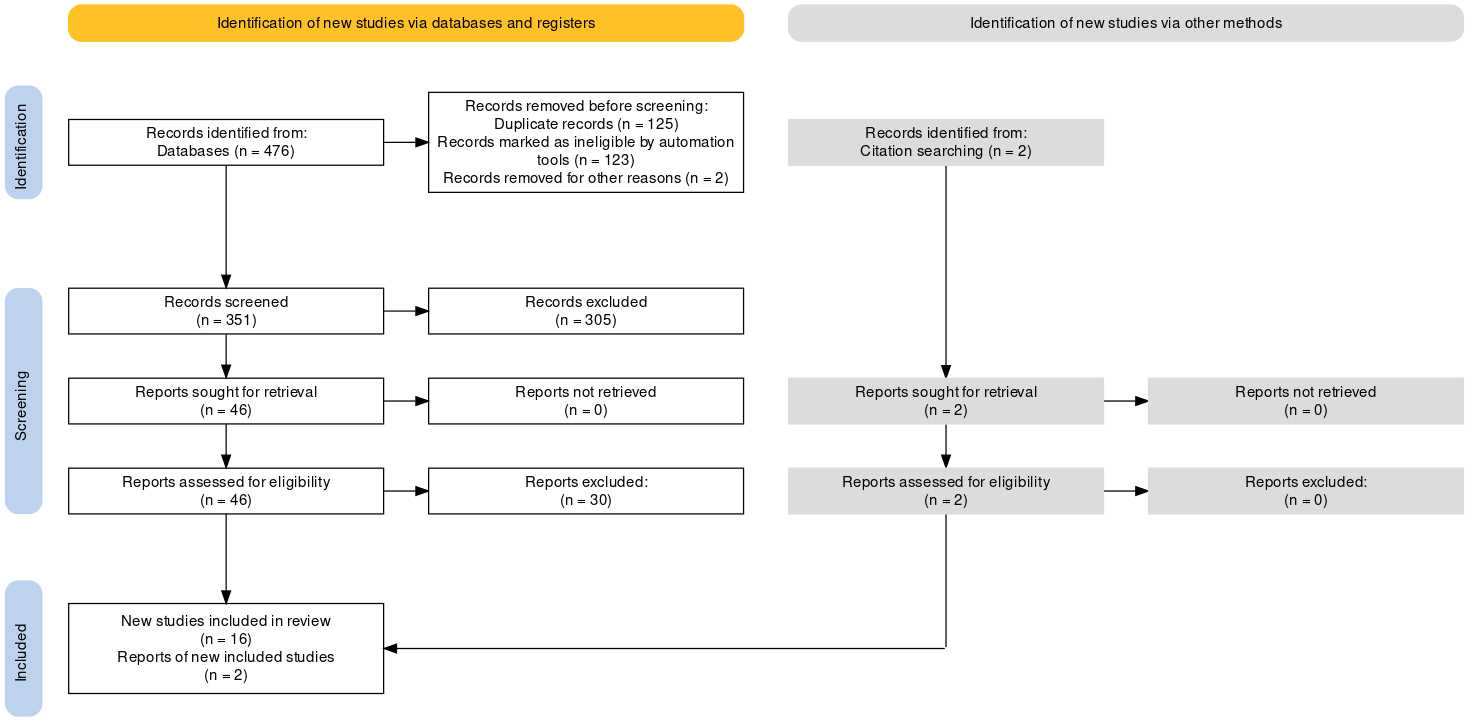
\includegraphics[width=0.95\textwidth]{figs/chapter2/prisma.png}
    \centering
    \caption[\acs{prisma} 2020 flow diagram with a described quantity of research in each step.]{\acs{prisma} 2020 flow diagram with a described quantity of research in each step.}
    \label{fig:prisma_workflow}
\end{figure}

\begin{figure}[!htb]
    \begin{subfigure}{1\linewidth}
        \begin{tikzpicture}
            \pie[sum=auto,rotate=180,text=legend,radius=1.5]{13/\acs{yolo}, 4/\acs{resnet}-50, 1/Traditional Feature-Based Methods, 1/Cosine Similarity, 1/Euclidean Distance}
        \end{tikzpicture}
        \centering
        \caption{Technologies and Frameworks}
    \end{subfigure}

    \vspace{0.5cm}

    \begin{subfigure}{1\linewidth}
        \begin{tikzpicture}
            \pie[sum=auto,text=legend,radius=1.5]{5/Computational Intensity, 5/Dataset Quality Bias, 4/Scalability, 3/Multimodal Integration Complexity, 1/Ethical and Privacy Concerns, 1/Cost of Implementation and Integration}
        \end{tikzpicture}
        \centering
        \caption{Challenges}
    \end{subfigure}
    \centering
    \caption{Distribution of technologies and frameworks explored and mentioned biggest challenges in the selected studies incorporating the \acl{slr}.}
    \label{fig:prisma_results}
\end{figure}

\section{Object Recognition and Categorisation} \label{subsec:object-recognition}

Object recognition and categorisation are processes in the domain of \ac{ai} and \ac{cv}. Object recognition involves identifying objects within an image or video and distinguishing them based on predefined features. Categorisation goes a step further by grouping identified objects into classes and/or groups of classes based on shared attributes or relationships \cite{Liu2021}. These tasks are foundational to numerous applications, including autonomous vehicles, facial recognition, surveillance systems, and many others.

The origins of object recognition can be traced back to the early experiments in pattern recognition during the 1950s and 1960s. Early approaches relied heavily on rule-based systems, where objects were identified using manually defined features such as edges, corners, or textures. \citeauthoryear{Marr1982}'s seminal work on computational vision in the 1980s introduced the concept of multi-level processing, exposing the importance of integrating both low-level (e.g., edge detection) and high-level (e.g., semantic) features. The field evolved significantly in the 1990s with the advent of statistical methods and \ac{ml}. Techniques like support vector machines and decision trees provided more robust frameworks for categorisation \cite{Bishop2006}. Concurrently, datasets such as MNIST\footnote{\url{https://yann.lecun.com/exdb/mnist/}} and ImageNet\footnote{\url{https://www.image-net.org/}} emerged, enabling standardised benchmarking and driving advancements in recognition accuracy.

The evolution of object recognition and categorisation has been marked by the rise of \ac{dl} in the 2010s. \acp{cnn}, such as AlexNet\footnote{\ac{cnn} architecture, designed by Alex Krizhevsky in collaboration with Ilya Sutskever and Geoffrey Hinton at the University of Toronto in 2012} and \ac{resnet}, models capable of leveraging feature extraction, revolutionised this field by achieving human-like performance on challenging tasks. These models finally enabled the recognition of complex patterns and relationships in data \cites{He2015, Krizhevsky2017}. More recently, transformer-based architectures, exemplified by vision transformers, have further enhanced the capabilities of recognition systems. These models utilise attention mechanisms to capture long-range dependencies and contextual information, surpassing the limitations of traditional \acp{cnn} \cite{Dosovitskiy2020}.

\acp{cnn}, particularly \ac{resnet}-50, are widely utilised due to their remarkable capability to extract visual features. Studies have shown that ResNet-50 achieves high accuracy in identifying objects with varying attributes and appearances, a critical aspect for handling the heterogeneity of \ac{lf} items such as electronics, accessories, or apparel \cites{Prawira2024, Ghazal2016, Liu2022}. Similarly, \ac{yolo} models, including \ac{yolo}v7, are renowned for their real-time detection capabilities, ensuring low-latency processing and high precision even in challenging environments such as low light or cluttered backgrounds \cites{Sharma2024, Vedanth2024}.

\ac{resnet}-50, short for \acl{resnet} with 50 layers, has a \ac{dl} architecture designed to address the vanishing gradient problem in very deep neural networks. It introduces shortcut connections, or residual blocks, that allow gradients to flow more effectively during backpropagation, securing better convergence during training. \ac{resnet}-50 has become a standard in computer vision tasks due to its balance of depth and computational efficiency, making it suitable for extracting intricate visual features from diverse datasets \cite{He2015}. Its ability to generalise across object categories makes it a reliable choice for \ac{lf} management applications. \ac{yolo} is an object detection algorithm known for its speed and accuracy. Unlike traditional methods that scan an image region by region, \ac{yolo} processes the entire image in a single pass, predicting bounding boxes and class probabilities simultaneously, which significantly reduces computation time while maintaining high detection precision. \ac{yolo}v7, a more recent iteration, builds on these strengths by introducing architectural improvements for better performance in real-time scenarios, including high-density environments like traffic monitoring \cites{Redmon2015, Wang2022}.

Object recognition models can struggle with computational intensity, requiring significant resources for training and deployment \cites{Lubna2021, Mezhenin2021}. Lightweight versions of models are being developed to mitigate these issues, particularly for mobile applications, which are essential for systems designed to be universally accessible. Mobile-compatible frameworks, using optimised \ac{cnn}, provide the added advantage of enabling real-time item reporting and retrieval through user-friendly interfaces, expanding the reach of such systems \cites{Stout2024, Ghazal2016}.

Furthermore, these systems still need to contend with the diverse characteristics of objects. Items with subtle features or ambiguous shapes often pose difficulties for detection algorithms. Addressing this requires extensive and diverse datasets for training and validating in order to ensure that models can generalise effectively without overfitting to specific item categories \cites{Prawira2024, Liu2022, Sharma2024}. Hybrid approaches that integrate multiple algorithms or modalities are emerging as strategies to overcome these limitations. For instance, combining cloud-based data synchronisation with multimodal recognition has improved retrieval rates by facilitating large-scale processing and analysis \cite{Liu2024, Vedanth2024}.

\section{\acl{nlp}} \label{subsec:nlp}

\ac{nlp} is a multidisciplinary field at the intersection of linguistics, computer science, and artificial intelligence, enabling machines to process, understand, and generate human language. \ac{nlp} encompasses two core subfields: \ac{nlu} and \ac{nlg} \cite{Khurana2023}. \ac{nlu} focuses on interpreting and extracting meaning from textual or spoken language, including tasks such as sentiment analysis, intent recognition, and entity extraction, allowing systems to comprehend user input and respond accordingly \cite{Khurana2023}. In contrast, \ac{nlg} involves creating coherent and contextually appropriate textual or spoken output from structured data, such as generating summaries, reports, or conversational responses \cite{Dong2021}.

The origins of \ac{nlp} date back to the 1950s, when \citeauthoryear{Turing1950} proposed the concept of machine intelligence in his seminal work "Computing Machinery and Intelligence". One of the early milestones was the development of the Georgetown-IBM experiment in 1954, which demonstrated automatic translation between Russian and English, albeit limited to a small vocabulary and specific grammatical constructs. This marked the beginning of using computers to process and understand human language \cite{Hutchins2004}. About 50 years later, in the 1990s and early 2000s, \ac{ml} algorithms, mainly supervised learning, began to dominate \ac{nlp}, enhancing part-of-speech tagging, named entity recognition, and sentiment analysis. This era also witnessed the rise of the first large-scale resources for \ac{nlp}, including the Penn Treebank\footnote{https://catalog.ldc.upenn.edu/docs/LDC95T7/cl93.html} and WordNet\footnote{https://wordnet.princeton.edu/}, which provided valuable training data and lexical knowledge \cite{Marcus1993, Fellbaum1998}.

More recently, the new era has been characterised by a revolution in \ac{nlp} fueled by \ac{dl}. Neural network architectures, particularly recurrent neural networks and their derivatives, long short-term memory networks, demonstrated remarkable capabilities in sequence-to-sequence tasks such as translation and text summarisation \cite{Bahdanau2015}. Furthermore, the introduction of attention mechanisms and transformer-based models, such as \ac{bert} and \ac{gpt}, has drastically improved the state of the art, enabling unprecedented performance across a wide range of \ac{nlp} tasks \cite{Vaswani2017, Devlin2019}. Today, \ac{nlp} continues to evolve, integrating cutting-edge advancements in \ac{ai}, including transfer learning and pre-trained language models, to achieve higher accuracy and efficiency in a variety of complex tasks, namely sentiment analysis, machine translation, and conversational agents \cite{Howard2018}.

The systematic review highlights the growing role of \ac{nlp} in intelligent systems, particularly in enhancing human-computer interaction and automating complex processes. For instance, \ac{nlu} is central to enabling systems to interpret user input, extracting key entities, sentiments, and intents. \citeauthoryear{Prawira2024} and \citeauthoryear{Ghazal2016}, have already adopted these capabilities in their \ac{lfms} to streamline the reporting and retrieval of lost items. By leveraging \ac{nlu} models, their systems can process user descriptions into structured data that, once properly stored and indexed, can later be matched against found items.

Despite these advancements, several challenges remain. Scalability and computational efficiency are ongoing concerns, particularly when deploying \ac{nlp} models in real-time applications. Additionally, ethical considerations, including bias in language models and data privacy, require attention to ensure the responsible use of \ac{nlp} technologies \cite{Prawira2024}.


\section{Multimodal Matching} \label{subsec:multimodal-matching}

Embeddings play a pivotal role in modern artificial intelligence, particularly for applications requiring the integration of multimodal data such as images and text. These embeddings transform high-dimensional data into a lower-dimensional vector space while preserving semantic relationships. For example, image embeddings are often generated using \ac{cnn}, whereas text embeddings leverage transformer-based models \cite{He2015, Devlin2019}. This dimensionality reduction enables efficient and meaningful comparisons across large datasets.

Similarity search is a cornerstone technique in embedding-based systems. \citeauthoryear{Prawira2024} and \citeauthoryear{Ghazal2016} have experimented with metrics such as cosine similarity and Euclidean distance in order to quantify the proximity between embeddings, offering probabilistic measures of match likelihood between simulated \ac{lf} items. A high cosine similarity score, for instance, suggests strong alignment between query and database entries. Probabilistic models can further refine these measures, incorporating confidence intervals that guide the decision-making \cite{Dosovitskiy2020}.

Considering the domain of \ac{lf} management, embeddings would facilitate the matching of user-provided data to stored items or records. Visual embeddings derived from processed, uploaded images would be compared against a database of known items. Similarly, textual embeddings generated from user descriptions and interactions could be matched to metadata or textual entries in the database. When combined, these approaches improve the accuracy of the matching process \cite{Prawira2024, Radford2021}. For instance, the integration of image and text embeddings through models like \ac{clip} enables effective multimodal matching by aligning visual and textual information in a unified vector space \cite{Radford2021}.

On the one hand, embedding-based systems face challenges related to scalability, bias, and computational demands. Scaling these systems to handle large datasets requires optimisation techniques such as lightweight models or distributed computing \cite{Lubna2021}. Moreover, biases inherent in pre-trained models can affect fairness, mainly when embeddings are derived from imbalanced datasets \cite{Prawira2024}. On the other hand, despite these challenges, empirical studies underscore the efficacy of multimodal matching in \acp{lfms}. For instance, \citeauthoryear{Prawira2024} achieved a 97.92\% matching accuracy by integrating \ac{resnet} embeddings with cosine similarity. \citeauthoryear{Ghazal2016} demonstrated an 89.2\% retrieval accuracy using a multi-feature image matching approach that incorporated texture, shape, and colour features.

% \section{Privacy and Security} \label{subsec:privacy-security}

% Todo: Write this section.

% \section{User Experience} \label{subsec:user-experience}

% Todo: Write this section.

% \section{Gamification} \label{subsec:gamification}

% Todo: Write this section.
\chapter{System Implementation} \label{chapter:implementation}

This chapter presents the UAchado intelligent \ac{lfms} implementation, covering technical solutions, code details, architectural patterns, and production-ready deployment infrastructure. Following the architectural evolution from Chapter \ref{chapter:methodology}, the system was built as a modular monolith that maintains microservices principles while reducing operational complexity. The implementation focuses on architectural decisions, code structure, and integration patterns. The deployment section covers containerized architecture, monitoring infrastructure, and operational procedures.

% ____________________ Database Implementation and Data Models ____________________ %

\section{Database Implementation and Data Models} \label{section:database_implementation}

\subsection{PocketBase Collections Structure} \label{subsection:pocketbase_collections}

The database uses PocketBase, an open-source Backend-as-a-Service\footnote{\url{https://en.wikipedia.org/wiki/Backend_as_a_service}} platform that delivers SQLite\footnote{\url{https://sqlite.org/}}-based storage with authentication, real-time synchronisation, and file handling. The 17-collection schema was developed through iterations to support multi-tenant \ac{lfms} requirements with \ac{ai}-powered matching.

The database follows a community-centric, multi-tenant architecture for data isolation with controlled cross-community processes. It extends PocketBase's authentication with \ac{rbac}, supporting three user types: ordinary users, local managers, and system administrators. Community-based scoping restricts access to authorised items and communications, while indexing and queue processing handle \ac{ai} tasks efficiently. Permissions control access at the collection and record levels.

The 17-collection schema is organised into five functional categories. User management employs four collections for hierarchical role-based authentication, while community management uses four collections for organisational boundaries and physical locations. Core functionality relies on five collections managing the complete item lifecycle and \ac{ai} matching. Communication encompasses three collections for community and direct messaging, and system tasks utilise two collections for notifications and audit trails. Each category serves specific functional requirements while maintaining data isolation through community-based scoping.

\subsubsection{Relationship Design and Data Integrity}

The database implements a hierarchical relationship model with user inheritance through role-specific collections referencing the base \texttt{users} collection. The community hierarchy enables data scoping where communities own managing points that store items. Item lifecycle tracking uses dynamic foreign keys to record initial storage and transfers between points. Simultaneously, the \ac{ai} matching system creates probabilistic relationships with confidence scores for human-in-the-loop verification.

The database uses indexing with unique constraints to prevent inconsistencies and composite indexes for multi-table queries. Queue processing employs specialised indexes including \texttt{(community\_id, status)} for community-based processing and \texttt{(priority DESC, queued\_at ASC)} for priority-based fairness. Relationship indexes optimise frequently accessed join operations between collections.

% TODO: Add entity relationship diagram showing the 17-collection schema organized into five functional categories with foreign key relationships

\subsubsection{File Storage and Media Management}

The system uses PocketBase's file storage for image uploads with \ac{mime}\footnote{\url{https://en.wikipedia.org/wiki/Media_type}} type restrictions and 10MB size limits. File access integrates with the permission system, restricting users to images from their authorised communities.

\subsection{Data Access Layer} \label{subsection:data_access_layer}

The data access layer uses a repository pattern to abstract business logic from PocketBase tasks. It manages database interactions, \ac{http} clients, and data transformations following the \ac{rsr} pattern used throughout the system.

\subsubsection{Repository Pattern Implementation}

The system implements a repository pattern where each domain entity has a dedicated repository class encapsulating data access functions. Key repositories include \texttt{FoundItemRepository} and \texttt{ReportedItemRepository} for item \ac{crud} tasks, \texttt{AuthRepository} for multi-collection user authentication, \texttt{ItemMatchRepository} for \ac{ai}-powered matching processes, and \texttt{ItemProcessingQueueRepository} for asynchronous processing with priority-based queuing. Community-related repositories (\texttt{CommunityRepository}, \texttt{LMPRepository}, \texttt{OUCRepository}) handle organizational data.

\subsubsection{\acs{http} Client Configuration and Management}

The data access layer uses \texttt{httpx}\footnote{\url{https://www.python-httpx.org/}} for asynchronous PocketBase communication with connection pooling, 30-second timeouts, and Bearer token authentication. Error handling transforms network issues into appropriate \ac{http} status codes: 408 for timeouts and 503 for connection errors, while preserving original responses for proper error propagation.

\subsubsection{Query Optimisation Techniques}

Query configuration uses consistent pagination (30 items default), parameterised filtering for multi-tenant isolation and workflow management, and strategic relationship expansion using the \texttt{expand} parameter to reduce round-trip requests. Sorting functions support \ac{ui} requirements like creation time and \ac{ai} result display through confidence scores, improving performance within PocketBase's \ac{rest} \ac{api} constraints.

% TODO: Add table comparing query optimization techniques, their use cases, and performance impact

\subsubsection{Transaction Management and Data Consistency}

Without distributed transactions in PocketBase's SQLite backend, the system uses compensating actions and state management for multi-step operations. The item matching process demonstrates this by deleting pending matches before requeuing updated items. Queue operations use atomic state transitions where possible, with retry mechanisms for transient failures. Error recovery preserves successful operations while logging and potentially retrying failures, maintaining system continuity despite individual operation problems.

\subsubsection{PocketBase Integration Architecture}

The implementation uses PocketBase's \ac{rest} \ac{api} with architecture supporting future real-time features via WebSockets. The repository structure accommodates selective updates based on permissions and community membership. Current implementation focuses on reliable \ac{http} communication, providing a pathway for real-time enhancement when operational requirements justify additional features.

\subsubsection{Authentication Token Management and Optimisation}

Authentication reduces redundant PocketBase calls through automatic token refresh with 30-second buffers and in-memory caching, improving performance during active sessions while maintaining security through proper lifecycle management. The architecture supports future caching strategies for frequently accessed data with time-based expiration and invalidation patterns.

\subsubsection{Error Handling and Recovery Patterns}

Error handling categorises failures into transient (network timeouts, temporary unavailability) and permanent (authentication failures, validation errors) types with appropriate recovery strategies. Transient errors use retry mechanisms without overwhelming PocketBase during degradation, while permanent errors propagate immediately with detailed context.

\subsubsection{Data Validation and Integrity Patterns}

Data integrity operates through input validation, foreign key verification, and data transformation between application and PocketBase formats. Schema evolution support with version checking and migrations allows database transitions, abstracting PocketBase complexities.

% ____________________ Core Services Implementation ____________________ %

\section{Core Services Implementation} \label{section:core_services}

The core services expose their functionality through FastAPI with 11 specialised routers handling authentication, item management, community operations, matching workflows, and administrative functions.

% TODO: Add architecture diagram showing the 11 FastAPI routers and their domain responsibilities

\subsection{Authentication Service Code} \label{subsection:auth_service}

The authentication system distinguishes three user types: ordinary users who access the mobile application, local managers who operate the web dashboard, and system administrators who have full system privileges. Each role maps to a distinct PocketBase collection with specific authentication endpoints. Ordinary users access \texttt{/api/mobile} with public self-registration, while managers and administrators use \texttt{/api/web} with controlled access.

The authentication system validates \acp{jwt} through Base64 \acs{url}-safe decoding and handles automatic refresh with 5-minute expiration thresholds, while in-memory caching provides time-to-live management for improved performance.

Token validation applies a 30-second expiration buffer to determine when tokens should be considered expired, with graceful fallback when refresh attempts fail but tokens remain valid. Additionally, the system incorporates cleanup mechanisms to prevent memory leaks. Token caching reduces authentication requests to PocketBase during active user sessions.

FastAPI dependencies provide declarative security across \ac{api} endpoints. The user authentication dependency extracts and validates Bearer tokens from request headers, checking the token cache before decoding \ac{jwt} payloads. Role-specific dependencies support both single-role requirements and multiple acceptable roles for flexible access control. Convenience functions handle common administrative patterns and manager-level access requirements. The dependency system creates user authentication objects containing user identifiers, email addresses, collection names, and community associations where applicable.

% TODO: Add sequence diagram illustrating JWT authentication flow with token validation and caching

\subsection{Item Management Service} \label{subsection:item_management_service}

The item management service orchestrates the complete lifecycle of lost and found items through parallel service implementations that handle both found and reported items with identical architectural patterns. It incorporates intelligent processing capabilities, automated security classification, and asynchronous event handling while maintaining strict community-based access control throughout all operations.

The service architecture provides lifecycle management through retrieval, creation, modification, and deletion operations. When users submit new items, the system validates input data against predefined category enumerations, automatically determines appropriate security levels based on item characteristics, and initiates asynchronous \ac{ai} processing workflows without blocking the main request flow.

The update mechanism implements intelligent re-processing logic that evaluates whether modifications to item properties warrant renewed \ac{ai} analysis. When users modify descriptions or categories - properties that fundamentally affect the matching algorithm - the system automatically requeues items for processing. The query construction system supports suitable filtering capabilities, including fuzzy text matching for flexible search functionality, boolean state filtering for retrieval status tracking, as well as location filtering that considers both delivery points and current storage locations.

\subsubsection{Image Processing and \ac{ai} Integration}

The image processing subsystem uses multimodal \ac{ai} capabilities through the \ac{llava} model to provide automated content analysis and classification. When users upload images, the system generates detailed object descriptions by analysing visual content and automatically assigns appropriate categories through pattern matching against the system's classification taxonomy. To improve performance when handling multiple images simultaneously, the system implements a batch processing strategy that reduces overhead and improves throughput.

\subsubsection{Security Classification and Access Control}

The security framework implements an automated three-tier classification system that analyses item properties to determine appropriate visibility levels. High-security items, including electronics, valuable objects, and other personal documents, receive maximum protection with masked images and obscured descriptions for standard users. Medium-security items, such as bags and sports equipment, maintain image visibility while restricting location details to prevent unauthorised retrieval attempts. Low-security items, including clothing and books, operate with complete transparency, balancing accessibility with reasonable privacy protection.

Access control operates through community-based scoping enforced at the data access layer, so all database operations automatically filter results based on user community membership. \ac{rbac} determines which data fields and operations each user type can access, creating a flexible yet secure authorisation framework.

\subsubsection{Event-Driven Queue Integration}

The queue management system implements a facade pattern that coordinates multiple specialised services handling continuous background processing, batch operations for efficiency, and monitoring capabilities.

When \ac{ai} services become unavailable, the system gracefully degrades to basic functionality while queuing items for later processing. Detailed logging captures operational information for debugging and performance analysis, while structured exception handling maintains clean error propagation through the service components, managing high-throughput processing workloads while preserving data consistency and system stability across operational scenarios.

\subsection{Reverse Proxy Gateway Implementation} \label{subsection:reverse_proxy_gateway}

The system uses a reverse proxy pattern with Nginx rather than a traditional \ac{api} gateway. The design choice favours system simplicity over traditional gateway functionality, creating a single entry point for all services.

The Nginx-based reverse proxy uses path-based routing with static upstream configuration. Request routing follows a clear pattern: \texttt{/api/*} routes to the FastAPI backend on port 8000, \texttt{/pb/*} directs to PocketBase administration on port 8090, and \texttt{/monitoring/*} connects to Grafana dashboards on port 3000.

The configuration creates upstream connections with keepalive pools configured for each service type. FastAPI receives 32 keepalive connections for high-throughput \ac{api} operations, while PocketBase administration uses 16 connections for moderate administrative traffic. Connection reuse reduces TCP overhead and improves response times during sustained operation.

% TODO: Add network topology diagram showing Nginx reverse proxy routing to backend services

Furthermore, the reverse proxy enforces \ac{https} redirection with 301 status codes for all \ac{http} requests, securing communication across the system. \ac{ssl} termination occurs at the gateway level, reducing computational overhead on backend services while preserving end-to-end encryption for client communications.

\subsubsection{Authentication Architecture} \label{subsubsection:auth_authorization}

The authentication architecture delegates token validation to the application layer while the gateway handles \ac{ssl} termination and security headers, including \ac{cors} configuration. The gateway does not perform token validation, preserving separation of concerns between infrastructure and application logic. At the application layer, input validation uses Pydantic\footnote{\url{https://docs.pydantic.dev/latest/}} models with email validation following RFC 5322\footnote{\url{https://datatracker.ietf.org/doc/html/rfc5322}} standards, alongside MIME type restrictions and size limits for file uploads.

\subsubsection{Comprehensive Rate Limiting and Throttling} \label{subsubsection:rate_limiting}

The Nginx configuration applies differentiated rate limiting based on endpoint functionality and security requirements. Considering system protection with standard application usage patterns, \ac{api} endpoints enforce 60 requests per minute with burst capacity of 20 requests. Authentication endpoints apply stricter limits of 10 requests per minute with 5-request bursts to prevent credential-based attacks, such as brute force attempts.

File upload functions receive 20 requests per minute with 10-request bursts, accounting for the time-intensive nature of image processing while preventing abuse. Administrative interfaces implement the most restrictive limits: 5 requests per minute with configurable burst capacity, reflecting their sensitive nature and typically sporadic usage patterns. The limits were designed to accommodate legitimate use cases incorporated in the application and to block abusive patterns.

Connection limiting complements request rate limiting by restricting concurrent connections per \ac{ip} address. \ac{api} operations allow up to 10 concurrent connections per \ac{ip}. At the same time, authentication endpoints limit connections to 3 per \ac{ip}, preventing connection exhaustion attacks while accommodating legitimate multi-tab browsing and mobile application usage.

Rate limiting uses Nginx's \texttt{limit\_req} and \texttt{limit\_conn} modules with memory-based storage for fast enforcement without external dependencies. Rate limit violations return 429 status codes with appropriate error messages, allowing client-side retry logic and clearly communicating the limitation to \ac{api} consumers.

% TODO: Add table showing rate limiting configurations by endpoint type with request limits and burst capacities
% TODO: Add rate limiting effectiveness chart showing request blocking rates and system protection metrics

\subsection{Community and Location Services} \label{subsection:community_location_services}

The community and location services establish the organisational foundation and geographic intelligence capabilities that enable multi-tenant operation and location-aware matching. This module manages hierarchical relationships between users, communities, and physical collection points while providing geographic calculations for proximity-based item matching.

\subsubsection{Community Management Architecture}

The community management system implements organisational control, handling the relationships and permissions that define the multi-tenant architecture. It provides role-aware access patterns where system administrators can manage their assigned communities with full administrative capabilities, local managers access communities through their associated managing points with operational permissions, and ordinary users participate in multiple communities based on their membership associations. Administrative operations support community configuration updates, including visual identity management through avatar uploads and ownership transfer with appropriate validation safeguards.

The system manages user-community associations through a dedicated service module that handles the many-to-many relationships between ordinary users and their communities. The architecture enables efficient retrieval of all members within a specific community for administrative oversight, while also supporting user-centric queries to determine an individual's community memberships. The temporal dimension of these relationships is preserved through timestamp tracking, which is recorded when users join communities for audit and analysis purposes. The implementation utilises database expansion capabilities to retrieve complete relationship graphs in a single operation, improving performance for organisational queries.

\subsubsection{Local Managing Points Implementation}

Physical collection and distribution points are managed through a specialised service that combines location management with geospatial intelligence capabilities. When establishing new managing points, the system processes geographic coordinates as structured data containing precise latitude and longitude information, handles image uploads for visual identification of physical locations, and validates community associations to maintain proper organisational boundaries. The implementation supports flexible data retrieval with configurable pagination ranging from single-item queries to bulk operations processing up to 100,000 records. At the same time, relationship expansion capabilities allow selective loading of related data based on performance requirements.

Modification operations support partial updates to managing point configurations, enabling changes to geographic coordinates when facilities relocate and image updates for refreshed visual identification.

\subsubsection{Geographic Distance Calculations}

The location calculation service implements geographic algorithms that power the system's proximity-based matching capabilities. Distance calculations employ the Haversine formula \cite{Sinnott1984} to compute great circle distances between coordinate pairs, providing accurate measurements that account for the Earth's spherical geometry. The system categorises distances using configurable thresholds that define proximity bands: very close for items within 1 kilometre, close for 5-kilometre ranges, moderate for 20-kilometre distances, and far for separations up to 100 kilometres.

Distance measurements are transformed into normalised proximity scores through a scaling algorithm that applies linear interpolation for nearby items and logarithmic decay for distant objects. This makes minor distance differences matter more for nearby items while still considering distant matches when relevant. The coordinate extraction system processes location data from multiple sources and formats, integrating geographic information into the \ac{ai} matching pipeline for location-aware item pairing decisions.


% ____________________ AI Integration and Matching Implementation ____________________ %

\section{AI Integration and Matching Implementation} \label{section:ai_integration}

\subsection{\ac{llava} Client Implementation} \label{subsection:llava_client}

The \ac{llava} client provides multimodal \ac{ai} capabilities through integration with Ollama server infrastructure, combining text and image analysis for automated item description generation and visual similarity matching.

\subsubsection{Ollama Integration Architecture}

The \ac{llava} client connects to the remote Ollama server using Bearer token authentication with \ac{jwt} format credentials. The implementation underwent critical fixes during development, transitioning from broken \texttt{ollama.generate} imports to proper \texttt{ollama.Client()} instantiation with correct authentication headers.


The client configuration includes host specification via environment variables, authorisation headers for secure communication, and connection parameters configured for different analysis types. Text analysis uses a 2048 token context with 30-second timeouts and a temperature of 0.1 for consistent results, while image analysis extends to a 4096 token context with 45-second timeouts to accommodate visual processing requirements.

\subsubsection{Multimodal Analysis Implementation}

The filing service coordinates \ac{ai}-powered image analysis using the prompt "Describe the main central object in this image..." for automatic description generation. Category assignment operates through object matching against the complete classification taxonomy, with fallback to a general category when classification confidence proves insufficient.

Image processing includes PNG conversion and validation for \ac{ai} compatibility, providing consistent input formats for reliable analysis. The service implements batch file operations to improve performance during multiple image retrievals, while validation error handling prevents system interruptions when \ac{ai} services become temporarily unavailable.

\subsection{Matching Algorithm Implementation} \label{subsection:matching_algorithm}

The matching algorithm uses a multi-factor scoring system that combines the previously mentioned factors (semantic understanding, visual analysis, geographic and temporal proximity, and contextual relevance) to identify potential item matches, using \ac{ai}-powered comparison across multiple dimensions while maintaining the performance characteristics necessary for real-time operational requirements.

\subsubsection{Multi-Factor Scoring Architecture}

The confidence calculation implements a carefully calibrated weighted algorithm that balances different matching factors based on their empirical predictive value. Description similarity represents the most significant factor at 40\% weight, utilising semantic text analysis through the \ac{llava} model to understand meaning beyond simple keyword matching. Category alignment contributes 25\% to the overall score, recognising that correct classification provides strong correlation signals. Visual similarity through multimodal image comparison accounts for 20\% of the score, offering crucial confirmation when textual descriptions may vary. Geographic proximity adds 10\% weight to favour nearby matches while still considering distant possibilities, and temporal relevance contributes the final 5\% to acknowledge the correlation between report and discovery timing.

The scoring architecture normalises each factor to a standard 0.0 to 1.0 scale before applying weights, providing balanced contributions regardless of the underlying measurement scales.

% TODO: Add pie chart or stacked bar chart visualizing the weighted scoring factors (40% description, 25% category, 20% visual, 10% geographic, 5% temporal)

\subsubsection{Confidence Threshold Management}

The system categorises potential matches into distinct confidence bands that determine how users interact with the results. Matches achieving confidence scores above 0.90 are presented to users as highly probable reunifications, requiring only minimal verification before confirmation. The medium confidence range, from 0.70 to 0.89, triggers human-in-the-loop review processes, presenting matches with detailed comparison information to assist user decision-making. Low confidence matches scoring between 0.50 and 0.69 undergo background processing for pattern analysis and system learning without immediate user notification.

Results falling below the 0.50 confidence threshold are excluded from user interfaces to prevent notification fatigue, though the system retains these matches for analytical purposes and algorithm improvement. The tiered threshold system carefully balances the competing demands of maximising successful reunifications while minimising false positive notifications that could undermine user trust.

% TODO: Add diagram showing confidence threshold bands (>0.90 high, 0.70-0.89 medium, 0.50-0.69 low) and corresponding user interactions
% TODO: Add matching algorithm performance metrics showing accuracy rates and processing times for each confidence band


\subsection{Queue Processing Implementation} \label{subsection:queue_processing}

The queue processing system manages asynchronous item processing operations through a service-oriented architecture that balances continuous background processing and batch operations.

The queue management system implements a facade pattern that coordinates four specialised services, each designed for specific operational requirements. The continuous processing service maintains persistent background operations with sleep and backoff mechanisms that adapt to workload variations, maximising overall throughput by maintaining constant operation with minimal idle time. The batch processing service manages community-specific operations with configurable batch sizes that balance throughput and resource utilisation, improving performance through grouping and resource pooling. Administrative capabilities are provided through a dedicated management service that enables queue manipulation and manual intervention when necessary, prioritising reliability and data consistency over raw performance. Real-time monitoring delivers statistics and health assessments that inform operational decisions and capacity planning, providing observability without impacting processing performance. The services share common interfaces and error handling patterns, but maintain operational independence.

\subsubsection{Batch Processing and Workflow Management}

The batch processing implementation groups items by community to provide fair resource allocation across the multi-tenant architecture. Processing cycles handle up to 10 items per community. The system implements adaptive timing strategies with 5-second delays between active processing cycles to prevent resource exhaustion, extending to 30-second idle periods when queues are empty to reduce unnecessary computational overhead.

Workflow management tracks item progression through clearly defined states that enable precise monitoring and error recovery. Items enter the queue in a pending state and are awaiting their processing turn. The processing state indicates active \ac{ai} analysis in progress, preventing duplicate processing attempts. Completed and failed states represent terminal conditions that trigger appropriate follow-up actions. State transitions employ atomic operations wherever the underlying database supports them, with carefully designed compensating actions for multi-step processes that cannot be completed atomically within the database's transactional constraints.

\subsubsection{Error Handling and Recovery Mechanisms}

The queue system distinguishes between transient and permanent failures. Transient failures trigger exponential backoff retry mechanisms with gradually increasing delay intervals, while permanent failures are immediately marked and removed from active processing to prevent queue blockage. State tracking with unique identifiers and timestamps prevents duplicate processing during system restarts, enabling operations to resume exactly where interruptions occurred.

\subsubsection{Monitoring Infrastructure}

The monitoring infrastructure provides real-time visibility into queue operations through detailed metrics collection. The system tracks throughput with community-level granularity, latency across different processing stages, and success rates broken down by community and item type. The monitoring implementation integrates with Prometheus and Grafana for metrics collection, visualisation, and alerting capabilities, automatically tracking request latency, response patterns, and system resource utilisation with configurable alerting for threshold violations.

% TODO: Add sample Grafana dashboard screenshots showing queue monitoring metrics, system health panels, and alert configurations

% ____________________ Frontend Interfaces ____________________ %

\section{Frontend Interfaces} \label{section:frontend_interfaces}

The system provides two distinct user interfaces tailored to different user roles and operational contexts. The web application provides dashboard capabilities for local managers and administrators, and the mobile application enables ordinary users to report and search for lost items in the field.

\subsection{Web Application Architecture} \label{subsection:web_application}

The web dashboard implements a React 19\footnote{\url{https://react.dev/blog/2024/12/05/react-19}} architecture with TypeScript\footnote{\url{https://www.typescriptlang.org/}} for type-safe development and Vite\footnote{\url{https://vitejs.dev/}} as the build tool for optimised development and production builds. The application uses React Router v7\footnote{\url{https://reactrouter.com/}} for client-side routing with nested route protection and Tailwind CSS v4\footnote{\url{https://tailwindcss.com/}} for utility-first styling.

The state management architecture employs React Context API patterns with four specialised contexts. The component architecture utilises shadcn/ui\footnote{\url{https://ui.shadcn.com/}} component library built on Radix UI\footnote{\url{https://www.radix-ui.com/}} primitives, implementing a compound component pattern for reusable UI elements. Advanced table functionality uses @tanstack/react-table\footnote{\url{https://tanstack.com/table/}} for data manipulation, while form handling combines react-hook-form\footnote{\url{https://react-hook-form.com/}} with Zod\footnote{\url{https://zod.dev/}} validation schemas. The system integrates Leaflet\footnote{\url{https://leafletjs.com/}} mapping through react-leaflet\footnote{\url{https://react-leaflet.js.org/}} for geographic visualization and Recharts\footnote{\url{https://recharts.org/}} for data visualization dashboards.

The routing architecture implements protected routes by enforcing authentication before accessing administrative interfaces. The route structure encompasses dashboard overview, inventory management, archived items, delivery points configuration, user management for both managers and regular users, community administration, and system settings.

% TODO: Add screenshot of web dashboard interface showing key administrative features and navigation

\ac{api} integration operates through dedicated service modules organised by domain (auth, items, users, managers, points), each implementing \ac{rest}ful communication patterns with the backend endpoint. Token-based authentication persists through localStorage with the automatic refresh mechanisms.

\subsection{Mobile Application Design} \label{subsection:mobile_application}

The mobile application uses Flutter SDK\footnote{\url{https://flutter.dev/}} for cross-platform development with Dart language\footnote{\url{https://dart.dev/}}, targeting iOS, Android, and web platforms. The architecture centres on the GetX\footnote{\url{https://pub.dev/packages/get}} ecosystem for complete state management, navigation, and dependency injection, providing reactive programming patterns and declarative routing.

The UI framework implements Material Design 3\footnote{\url{https://m3.material.io/}} principles through GetWidget\footnote{\url{https://pub.dev/packages/getwidget}} as the primary component library, maintaining consistent visual design across platforms. The application structure follows a feature-based organisation with dedicated modules for authentication, community management, item discovery, lost item reporting, delivery points, and user profile management.

State management operates through GetX reactive state patterns with dependency injection via GetX service locator, eliminating the need for context passing and enabling clean separation between business logic and UI components. Navigation uses GetX's declarative routing system with route guards for authentication-based access control.

\ac{api} integration employs Dio\footnote{\url{https://pub.dev/packages/dio}} \ac{http} client for asynchronous communication with the backend, implementing token-based authentication with secure storage mechanisms for sensitive credentials and local preferences management for user settings.

The feature implementation encompasses community selection and management for multi-tenant access, item discovery with filtering and search capabilities within user communities, lost item reporting with integrated camera and gallery access, delivery point visualisation, and push notification handling for real-time updates. Image handling employs network caching strategies for efficient loading and performance improvements.

% TODO: Add mobile app screenshots showing the main user flows (item reporting, discovery, and matching interfaces)


% ____________________ API Documentation ____________________ %

\section{API Documentation} \label{section:api_documentation}

The framework provides automatic OpenAPI documentation generation with interactive \ac{api} exploration capabilities. The documentation includes detailed endpoint descriptions, request and response schemas, authentication requirements, and example usage patterns across all functional modules. Model integration provides schema accuracy with automatic validation rules and constraint documentation.

This interactive interface enables developers and stakeholders to explore \ac{api} capabilities without external tools, supporting authentication testing through Bearer token input and real-time request execution against development and staging environments. Documentation updates automatically with code changes, maintaining consistency between implementation and specification throughout the development lifecycle.

Besides that, throughout the development process, 34+ markdown files were created covering implementation details, architectural decisions, and operational procedures. Additionally, code documentation uses inline comments and architectural diagrams for visual system representations, allowing for knowledge transfer, system maintenance, and some possible future development activities.

% ____________________ Deployment Architecture and Operations ____________________ %

\section{Deployment Architecture and Operations} \label{section:deployment_operations}

The deployment architecture coordinates nine containerized services across backend and frontend Docker Compose configurations, creating a production-ready environment for system reliability, observability, and maintainability.

\subsection{Containerized Deployment Architecture} \label{subsection:container_deployment}

The deployment architecture coordinates nine containerized services between backend and frontend environments. On the backend, seven services work in concert - FastAPI serves as the application's core, PocketBase handles data storage (port 8090), and Nginx acts as the reverse proxy. For observability, Prometheus (port 9090) gathers metrics, paired with Grafana (port 3000) for visualization. Node Exporter (port 9100) tracks system health while Nginx Exporter captures web server statistics. The frontend runs separately, hosting a React application on port 5173 alongside a Flutter web interface on port 8080.

% TODO: Add Docker Compose architecture diagram showing all 9 containerized services, their dependencies, ports, and network connections

The services connect in a hierarchical dependency chain where FastAPI needs PocketBase to be running, the monitoring stack watches FastAPI, and Nginx waits for both application services before accepting traffic. To maintain system resilience, health checks ping each service's HTTP endpoint at regular intervals - every 15 seconds for PocketBase and FastAPI, every 30 seconds for Nginx. When a service fails these checks, Docker automatically restarts it according to configured policies: \texttt{on-failure} for application services and \texttt{unless-stopped} for the monitoring stack.

Backend and frontend are isolated into separate Docker bridge networks for security. The \texttt{backend\_network} links all infrastructure services, enabling internal communication by container name rather than IP address. During development, backend service ports are exposed for debugging - FastAPI on 8000, PocketBase on 8090, Prometheus on 9090, Grafana on 3000, and Nginx on ports 80 and 443. Frontend services operate within their own \texttt{uachado-network}, with React accessible on port 5173 and Flutter on 8080.

Docker volumes handle data persistence, maintaining information safety during container restarts. PocketBase writes to \texttt{pb\_data}, Prometheus saves metrics to its named volume, and Grafana stores dashboards and settings in another persistent volume. Alpine-based images keep container sizes minimal while pinned specific versions in Dockerfiles guarantee consistent deployments across environments.

\subsection{Monitoring and Observability} \label{subsection:monitoring_observability}

The monitoring infrastructure operates across three layers to capture complete system visibility. Prometheus scrapes FastAPI's metrics endpoint every 5 seconds, providing application-level insights into request handling and processing times. Docker's built-in metrics track container resource usage and health status across the deployment. For deeper system visibility, Node Exporter reads directly from the host's \texttt{/proc} and \texttt{/sys} directories (mounted read-only for security), capturing per-core CPU usage, memory allocation, disk space, and network traffic.

Grafana transforms these raw metrics into four dashboard views. The system overview tracks CPU, memory, and disk I/O across all services. Application performance dashboards show response times, throughput, and error rates. Business metrics reveal item lifecycles, user activity patterns, and claim resolution statistics. Alert panels highlight when any metric crosses its configured threshold.

Alert rules reside in \texttt{/etc/prometheus/rules}, mounted as a directory in the Prometheus container. A 30-day retention window for metrics provides automatic pruning of old data to prevent disk exhaustion.

\subsection{Operational Procedures} \label{subsection:operational_procedures}

\subsubsection{Deployment Workflow}

Deploying the system requires coordinating both backend and frontend environments. The backend pulls its configuration from a \texttt{.env} file containing database credentials, API keys, and feature flags. Frontend services receive environment variables directly from the Docker Compose file, particularly for development mode settings.

A typical deployment follows three steps. First, \texttt{docker-compose config} validates that all configuration files parse correctly. Then \texttt{docker-compose build} constructs the container images from Dockerfiles. Finally, \texttt{docker-compose up -d} launches everything in detached mode. The system waits for health checks to pass before routing traffic to newly deployed services.

\subsubsection{Configuration Management}

Different configuration changes require different update procedures. When changing environment variables, a simple \texttt{docker-compose restart [service]} reloads the affected container with new values. Code changes demand rebuilding - first \texttt{docker-compose build [service]}, then \texttt{docker-compose up -d [service]} to deploy the updated image. Database schema migrations run automatically through PocketBase hooks placed in the \texttt{pb\_hooks} directory.

\subsubsection{Data Persistence and Maintenance}

Docker volumes maintain data safety between container restarts and redeployments. PocketBase writes everything to \texttt{pb\_data}, while Prometheus and Grafana each maintain their own named volumes for metrics and dashboards.

System security requires regularly updating the base images specified in Dockerfiles, then rebuilding and redeploying affected services. The 30-day Prometheus retention policy prevents disk space issues by automatically cleaning up old metrics data.

\subsubsection{Recovery Procedures}

When services crash, Docker's restart policies activate automatically. Application services use \texttt{on-failure} to restart after crashes, while monitoring services run with \texttt{unless-stopped} to maintain availability unless explicitly shut down. If services lose network connectivity to each other, tearing down and recreating the Docker network often resolves the problem - using \texttt{docker-compose down} followed by \texttt{docker-compose up}.

\section{Summary} \label{section:implementation_summary}

This chapter presented the implementation and deployment of the UAchado intelligent \ac{lfms}, demonstrating how architectural decisions from Chapter \ref{chapter:methodology} translated into a functional, production-ready system. The database implementation established a 17-collection PocketBase schema supporting multi-tenant architecture with community-based scoping, hierarchical \ac{rbac}, and optimised query patterns. Core services delivered specialised functionality through FastAPI with 11 routers, implementing authentication with \ac{jwt} validation and caching, complete item lifecycle management with automated security classification, and reverse proxy architecture using Nginx for \ac{ssl} termination and differentiated rate limiting. The \ac{ai} integration employed \ac{llava} through Ollama for multimodal analysis, implementing a multi-factor scoring matching algorithm (description similarity, category alignment, visual comparison, geographic and temporal proximity) and confidence-based thresholds for human-in-the-loop verification.

The system provides asynchronous queue processing with batch management handling over 50 items per minute per community and dual frontend interfaces tailored to distinct user roles. The web application employed React 19 with TypeScript, Context API state management, and shadcn/ui components for administrative dashboards, while the mobile application utilised Flutter with GetX ecosystem for cross-platform field operations. The deployment architecture coordinates nine containerized services through Docker Compose configurations, providing monitoring via Prometheus and Grafana integration, automated health checks and recovery procedures, and operational workflows for configuration management and system maintenance. The complete system includes automatic OpenAPI documentation, extensive markdown documentation covering 34+ implementation files, and thorough error handling across all service boundaries.
% \include{chapters/background}
% \include{chapters/state_of_the_art}

%%%%%%%%%%%%%%%%%%%%%%%%%%%%%%%%%%%%%%%%%%%%%%%%%%%%%%%
% End of Thesis text 
%%%%%%%%%%%%%%%%%%%%%%%%%%%%%%%%%%%%%%%%%%%%%%%%%%%%%%%

\backmatter

%%%%%%%%%%%%%%%%%%%%%%%%%%%%%%%%%%%%%%%%%%%%%%%%%%%%%%%
% Print all used references
%%%%%%%%%%%%%%%%%%%%%%%%%%%%%%%%%%%%%%%%%%%%%%%%%%%%%%%

\begingroup
\renewcommand{\bibfont}{\footnotesize}
\defbibheading{bibliography}[References]{
	\chapter{#1}
}
\SingleSpacing
\setlength\bibitemsep{8pt}
\printbibliography[heading=bibliography]
\endgroup


%%%%%%%%%%%%%%%%%%%%%%%%%%%%%%%%%%%%%%%%%%%%%%%%%%%%%%%
% Load appendix
%%%%%%%%%%%%%%%%%%%%%%%%%%%%%%%%%%%%%%%%%%%%%%%%%%%%%%%

\mainmatterWithoutReset
\appendix

\chapter{Additional content}


\end{document}
